\chapter{Calculus and Mathematical Analysis}

\section{Function}

\subsection{Function Definition}

\begin{exercise}
Given \( f(x) = \frac{1-x}{1+x} \), find the values of \( f(0) \), \( f(-x) \), \( f(x+1) \), \( f(x) + 1 \), and \( f\left( \frac{1}{x} \right) \).
\end{exercise}
\begin{solution}
First, we calculate \( f(0) \):
\[
f(0) = \frac{1-0}{1+0} = \frac{1}{1} = 1
\]

Next, we find \( f(-x) \):
\[
f(-x) = \frac{1-(-x)}{1+(-x)} = \frac{1+x}{1-x}
\]

Then, we determine \( f(x+1) \):
\[
f(x+1) = \frac{1-(x+1)}{1+(x+1)} = \frac{1-x-1}{1+x+1} = \frac{-x}{x+2}
\]

Next, we compute \( f(x) + 1 \):
\[
f(x) + 1 = \frac{1-x}{1+x} + 1 = \frac{1-x + 1+x}{1+x} = \frac{2}{1+x}
\]

Finally, we find \( f\left( \frac{1}{x} \right) \):
\[
f\left( \frac{1}{x} \right) = \frac{1 - \frac{1}{x}}{1 + \frac{1}{x}} = \frac{\frac{x-1}{x}}{\frac{x+1}{x}} = \frac{x-1}{x+1}
\]
\end{solution}

\begin{exercise}
Find the domain of the following functions:
\begin{enumerate}
    \item \( y = (x-2) \sqrt{\frac{1+x}{1-x}} \)
    \item \( y = \sqrt{\cos x^2} \)
    \item \( y = \frac{\sqrt{x}}{\sin \pi x} \)
    \item \( y = \arcsin \frac{2x}{1+x} \)
    \item \( y = \arcsin (1-x) + \lg (\lg x) \)
\end{enumerate}
\end{exercise}

\begin{solution}
The domains of the given functions are as follows:
\begin{enumerate}
    \item For \( y = (x-2) \sqrt{\frac{1+x}{1-x}} \):
    \begin{itemize}
        \item The square root function requires the argument to be non-negative: \( \frac{1+x}{1-x} \geq 0 \).
        \item The denominator \( 1-x \) must be positive (to avoid division by zero and ensure the expression inside the square root is defined):
        \[
        1-x > 0 \implies x < 1
        \]
        \item Combining these conditions, we have:
        \[
        -1 \leq x < 1
        \]
    \end{itemize}
    
    \item For \( y = \sqrt{\cos x^2} \):
    \begin{itemize}
        \item The argument of the square root must be non-negative: \( \cos x^2 \geq 0 \).
        \item Cosine function is non-negative when \( x^2 \) lies within intervals where cosine is non-negative:
        \[
        \cos x^2 \geq 0 \implies x^2 \in \left[2k\pi - \frac{\pi}{2}, 2k\pi + \frac{\pi}{2}\right] \quad \text{for integer } k.
        \]
        \item Solving for \( x \):
        \[
        x \in \left[-\sqrt{2k\pi + \frac{\pi}{2}}, \sqrt{2k\pi + \frac{\pi}{2}}\right]
        \]
    \end{itemize}

    \item For \( y = \frac{\sqrt{x}}{\sin \pi x} \):
    \begin{itemize}
        \item The numerator \( \sqrt{x} \) requires \( x \geq 0 \).
        \item The denominator \( \sin \pi x \) must be non-zero:
        \[
        \sin \pi x \neq 0 \implies x \notin \mathbb{Z}
        \]
        \item Combining these conditions, we have:
        \[
        x \geq 0 \quad \text{and} \quad x \notin \mathbb{Z}
        \]
    \end{itemize}

    \item For \( y = \arcsin \frac{2x}{1+x} \):
    \begin{itemize}
        \item The argument of the arcsine function must lie within \([-1, 1]\):
        \[
        -1 \leq \frac{2x}{1+x} \leq 1
        \]
        \item Solving the inequalities:
        \[
        \frac{2x}{1+x} \leq 1 \implies 2x \leq 1 + x \implies x \leq 1
        \]
        \[
        \frac{2x}{1+x} \geq -1 \implies 2x \geq -1 - x \implies x \geq -\frac{1}{3}
        \]
        \item Combining these conditions, we have:
        \[
        -\frac{1}{3} \leq x \leq 1
        \]
    \end{itemize}

    \item For \( y = \arcsin (1-x) + \lg (\lg x) \):
    \begin{itemize}
        \item The argument of the arcsine function must lie within \([-1, 1]\):
        \[
        -1 \leq 1-x \leq 1 \implies 0 \leq x \leq 2
        \]
        \item The argument of the logarithmic function must be positive:
        \[
        \lg x > 0 \implies x > 1
        \]
        \item Combining these conditions, we have:
        \[
        1 < x \leq 2
        \]
    \end{itemize}
\end{enumerate}
\end{solution}

\begin{exercise}
Find the domain and range of the following functions:
\begin{enumerate}
    \item \( y = \sqrt{2 + x - x^2} \)
    \item \( y = \arccos \frac{2x}{1+x^2} \)
    \item \( y = \sqrt{x - x^2} \)
\end{enumerate}
\end{exercise}
\begin{remark}
    Given a quadratic function \( f(x) = ax^2 + bx + c \):

\begin{enumerate}
    \item Determine the direction of the parabola:
    \begin{itemize}
        \item If \( a > 0 \), the parabola opens upwards and \( f(x) \) has a minimum value.
        \item If \( a < 0 \), the parabola opens downwards and \( f(x) \) has a maximum value.
    \end{itemize}

    \item Find the vertex:
    \begin{itemize}
        \item The \( x \)-coordinate of the vertex is \( h = -\frac{b}{2a} \).
        \item The \( y \)-coordinate of the vertex (the extremum value) is \( k = f(h) = c - \frac{b^2}{4a} \).
    \end{itemize}
    
    \item Conclusion:
    \begin{itemize}
        \item If \( a > 0 \), the minimum value of \( f(x) \) is \( k = c - \frac{b^2}{4a} \).
        \item If \( a < 0 \), the maximum value of \( f(x) \) is \( k = c - \frac{b^2}{4a} \).
    \end{itemize}
\end{enumerate}
\end{remark}
\begin{solution}
The domains and ranges of the given functions are as follows:
\begin{enumerate}
    \item For \( y = \sqrt{2 + x - x^2} \):
    \begin{itemize}
        \item The argument of the square root must be non-negative:
        \[
        2 + x - x^2 \geq 0
        \]
        \item This is a quadratic inequality, solving for \( x \):
        \[
        x^2 - x - 2 \leq 0 \implies (x-2)(x+1) \leq 0
        \]
        \item The solutions are:
        \[
        -1 \leq x \leq 2
        \]
        \item The range of \( y \) is determined by the maximum value of \( 2 + x - x^2 \) within the domain. The maximum value occurs at \( x = \frac{1}{2}(2+1) = 1.5 \):
        \[
        y_{\max} = \sqrt{2 + 1.5 - 1.5^2} = \sqrt{\frac{9}{4}} = \frac{3}{2}
        \]
        \item Therefore:
        \[
        0 \leq y \leq \frac{3}{2}
        \]
    \end{itemize}

    \item For \( y = \arccos \frac{2x}{1+x^2} \):
    \begin{itemize}
        \item The argument of the arcsine function must lie within \([-1, 1]\):
        \[
        -1 \leq \frac{2x}{1+x^2} \leq 1
        \]
        \item This inequality holds for all \( x \in \mathbb{R} \).
        \item The range of the \( \arccos \) function is:
        \[
        0 \leq y \leq \pi
        \]
    \end{itemize}

    \item For \( y = \sqrt{x - x^2} \):
    \begin{itemize}
        \item The argument of the square root must be non-negative:
        \[
        x - x^2 \geq 0
        \]
        \item This is a quadratic inequality, solving for \( x \):
        \[
        x(1 - x) \geq 0
        \]
        \item The solutions are:
        \[
        0 \leq x \leq 1
        \]
        \item The range of \( y \) is determined by the maximum value of \( x - x^2 \) within the domain. The maximum value occurs at \( x = \frac{1}{2} \):
        \[
        y_{\max} = \sqrt{\frac{1}{4}} = \frac{1}{2}
        \]
        \item Therefore:
        \[
        0 \leq y \leq \frac{1}{2}
        \]
    \end{itemize}
\end{enumerate}
\end{solution}

\begin{exercise}
\begin{enumerate}
    \item Given \( f\left( x + \frac{1}{x} \right) = x^2 + \frac{1}{x^2} \), find \( f(x) \).
    \item Given \( f\left( \frac{1}{x} \right) = x + \sqrt{1 + x^2} \) for \( x > 0 \), find \( f(x) \).
\end{enumerate}
\end{exercise}
\begin{solution}
\begin{enumerate}
    \item For the function \( f\left( x + \frac{1}{x} \right) = x^2 + \frac{1}{x^2} \), we need to find \( f(x) \).
    \begin{itemize}
        \item Let \( t = x + \frac{1}{x} \). Then we have:
        \[
        f(t) = x^2 + \frac{1}{x^2}
        \]
        \item We express \( x^2 + \frac{1}{x^2} \) in terms of \( t \):
        \[
        t^2 = \left( x + \frac{1}{x} \right)^2 = x^2 + 2 + \frac{1}{x^2}
        \]
        \item Thus, we get:
        \[
        x^2 + \frac{1}{x^2} = t^2 - 2
        \]
        \item Therefore:
        \[
        f(t) = t^2 - 2
        \]
        \item Hence, the function is:
        \[
        f(x) = x^2 - 2
        \]
    \end{itemize}

    \item For the function \( f\left( \frac{1}{x} \right) = x + \sqrt{1 + x^2} \) where \( x > 0 \), we need to find \( f(x) \).
    \begin{itemize}
        \item Let \( t = \frac{1}{x} \). Then:
        \[
        f(t) = x + \sqrt{1 + x^2}
        \]
        \item Substituting \( x = \frac{1}{t} \), we get:
        \[
        f(t) = \frac{1}{t} + \sqrt{1 + \left( \frac{1}{t} \right)^2} = \frac{1}{t} + \sqrt{\frac{t^2 + 1}{t^2}} = \frac{1}{t} + \frac{\sqrt{t^2 + 1}}{t} = \frac{1 + \sqrt{t^2 + 1}}{t}
        \]
        \item Thus:
        \[
        f(x) = \frac{1 + \sqrt{x^2 + 1}}{x}
        \]
    \end{itemize}
\end{enumerate}
\end{solution}



\begin{exercise}
In the open interval \(0 < x < 1\) on the \(O x\) axis, there is a uniformly distributed mass of \(2 \mathrm{~kg}\). At the points \(x = 2\) and \(x = 3\), there are concentrated masses of \(1 \mathrm{~kg}\) each. Let \(m(x)\) be the total mass in the interval \((-\infty, x)\). Find the analytical expression for the function \(m(x)\) in terms of a piecewise function and plot this function.
\end{exercise}
\begin{solution}
First, determine the expression for \( m(x) \) in different intervals:

1. For \( x \leq 0 \): There is no mass in the interval \((-\infty, x)\):
   \[
   m(x) = 0
   \]

2. For \( 0 < x \leq 1 \): The mass is uniformly distributed in the interval \( 0 < x < 1 \) with a total mass of \(2 \mathrm{~kg}\):
   \[
   m(x) = 2x
   \]

3. For \( 1 < x \leq 2 \): The entire \(2 \mathrm{~kg}\) mass in the interval \( 0 < x < 1 \) is considered:
   \[
   m(x) = 2 \mathrm{~kg}
   \]

4. For \( 2 < x \leq 3 \): In addition to the \(2 \mathrm{~kg}\) mass, there is a concentrated mass of \(1 \mathrm{~kg}\) at \( x = 2 \):
   \[
   m(x) = 3 \mathrm{~kg}
   \]

5. For \( x > 3 \): There are concentrated masses of \(1 \mathrm{~kg}\) each at \( x = 2 \) and \( x = 3 \):
   \[
   m(x) = 4 \mathrm{~kg}
   \]

The piecewise function \( m(x) \) can be written as:
\[
m(x) =
\begin{cases}
0, & x \leq 0 \\
2x, & 0 < x \leq 1 \\
2, & 1 < x \leq 2 \\
3, & 2 < x \leq 3 \\
4, & x > 3
\end{cases}
\]

\begin{center}
\begin{tikzpicture}
    \begin{scope}[xshift=0cm]
        \draw[->] (-1,0) -- (5,0) node[right] {$x$};
        \draw[->] (0,-1) -- (0,5) node[above] {$m(x)$};
        
        % Drawing the mass function
        \draw[thick, domain=-1:0] plot (\x, {0}) node[right] {};
        \draw[thick, domain=0:1] plot (\x, {2*\x}) node[right] {};
        \draw[thick] (1,2) -- (2,2) node[right] {};
        %\draw[thick] (2,2) -- (2,3) node[right] {};
        \draw[thick] (2,3) -- (3,3) node[right] {};
        %\draw[thick] (3,3) -- (3,4) node[right] {};
        \draw[thick, domain=3:5] plot (\x, {4}) node[right] {};
        
        % Adding the points
        \filldraw[black] (0,0) circle (2pt);
        \filldraw[black] (1,2) circle (2pt);
        \draw[fill=white] (2,2) circle (2pt);
        \filldraw[black] (2,3) circle (2pt);
        \draw[fill=white] (3,3) circle (2pt);
        \filldraw[black] (3,4) circle (2pt);

        % Adding labels
        \node at (1,-0.3) {$1$};
        \node at (2,-0.3) {$2$};
        \node at (3,-0.3) {$3$};
        \node at (-0.3,2) {$2$};
        \node at (-0.3,3) {$3$};
        \node at (-0.3,4) {$4$};
    \end{scope}
    
   
\end{tikzpicture}
\end{center}

\end{solution}

\begin{exercise}
Let \( f(x) \) be defined as follows:
\[
f(x) =
\begin{array}{ll}
1, & \text{if } |x| \leq 1 \\
0, & \text{if } |x| > 1
\end{array}
\]
Find \( f(f(x)) \).
\end{exercise}
\begin{solution}
We need to find the expression for \( f(f(x)) \).

First, consider the given function \( f(x) \):
\[
f(x) =
\begin{array}{ll}
1, & \text{if } |x| \leq 1 \\
0, & \text{if } |x| > 1
\end{array}
\]

We will analyze \( f(f(x)) \) by considering the two possible cases for \( f(x) \):

1. When \( |x| \leq 1 \):
   \[
   f(x) = 1
   \]
   Substituting \( f(x) = 1 \) into \( f \):
   \[
   f(f(x)) = f(1)
   \]
   Since \( 1 \) satisfies \( |1| \leq 1 \):
   \[
   f(1) = 1
   \]
   Therefore, when \( |x| \leq 1 \):
   \[
   f(f(x)) = 1
   \]

2. When \( |x| > 1 \):
   \[
   f(x) = 0
   \]
   Substituting \( f(x) = 0 \) into \( f \):
   \[
   f(f(x)) = f(0)
   \]
   Since \( 0 \) satisfies \( |0| \leq 1 \):
   \[
   f(0) = 1
   \]
   Therefore, when \( |x| > 1 \):
   \[
   f(f(x)) = 1
   \]

In both cases, we have \( f(f(x)) = 1 \). Hence, the function \( f(f(x)) \) is:
\[
f(f(x)) = 1
\]

\end{solution}

\begin{exercise}
Let \( f_n(x) = \underbrace{f(f(\cdots f(x)))}_{n \text{ times}} \). Given \( f(x) = \frac{x}{\sqrt{1+x^2}} \), find \( f_n(x) \).
\end{exercise}

\begin{solution}
First, we calculate \( f(f(x)) \):
\[
f(f(x)) = f\left( \frac{x}{\sqrt{1 + x^2}} \right)
\]
Substituting the definition of \( f \):
\[
f\left( \frac{x}{\sqrt{1 + x^2}} \right) = \frac{\frac{x}{\sqrt{1 + x^2}}}{\sqrt{1 + \left( \frac{x}{\sqrt{1 + x^2}} \right)^2}} = \frac{\frac{x}{\sqrt{1 + x^2}}}{\sqrt{\frac{1 + 2x^2}{1 + x^2}}} = \frac{x}{\sqrt{1 + 2x^2}}
\]

Thus,
\[
f(f(x)) = \frac{x}{\sqrt{1 + 2x^2}}
\]

Next, we calculate \( f(f(f(x))) \):
\[
f(f(f(x))) = f\left( \frac{x}{\sqrt{1 + 2x^2}} \right) = \frac{x}{\sqrt{1 + 3x^2}}
\]

From the pattern observed, we can generalize:
\[
f_n(x) = \frac{x}{\sqrt{1 + nx^2}}
\]

We will use mathematical induction to prove:
\[
f_n(x) = \frac{x}{\sqrt{1 + nx^2}}
\]

\textbf{Base Case:} For \( n = 1 \):
\[
f_1(x) = f(x) = \frac{x}{\sqrt{1 + x^2}}
\]
Clearly,
\[
f_1(x) = \frac{x}{\sqrt{1 + 1 \cdot x^2}} = \frac{x}{\sqrt{1 + x^2}}
\]
Thus, the proposition holds for \( n = 1 \).

\textbf{Induction Hypothesis:} Assume the proposition holds for \( n = k \), i.e.,
\[
f_k(x) = \frac{x}{\sqrt{1 + kx^2}}
\]

\textbf{Inductive Step:} We need to prove that the proposition holds for \( n = k+1 \), i.e.,
\[
f_{k+1}(x) = \frac{x}{\sqrt{1 + (k+1)x^2}}
\]

By definition,
\[
f_{k+1}(x) = f(f_k(x))
\]
Substitute the induction hypothesis:
\[
f_{k+1}(x) = f\left( \frac{x}{\sqrt{1 + kx^2}} \right)
\]
Using the definition of \( f(x) \):
\[
f\left( \frac{x}{\sqrt{1 + kx^2}} \right) = \frac{\frac{x}{\sqrt{1 + kx^2}}}{\sqrt{1 + \left( \frac{x}{\sqrt{1 + kx^2}} \right)^2}}
\]
Simplify the expression inside the square root:
\[
\left( \frac{x}{\sqrt{1 + kx^2}} \right)^2 = \frac{x^2}{1 + kx^2}
\]
Thus,
\[
1 + \left( \frac{x}{\sqrt{1 + kx^2}} \right)^2 = 1 + \frac{x^2}{1 + kx^2} = \frac{1 + kx^2 + x^2}{1 + kx^2} = \frac{1 + (k+1)x^2}{1 + kx^2}
\]
Therefore,
\[
f\left( \frac{x}{\sqrt{1 + kx^2}} \right) = \frac{\frac{x}{\sqrt{1 + kx^2}}}{\sqrt{\frac{1 + (k+1)x^2}{1 + kx^2}}} = \frac{x}{\sqrt{1 + (k+1)x^2}}
\]

So,
\[
f_{k+1}(x) = \frac{x}{\sqrt{1 + (k+1)x^2}}
\]

This shows that if the proposition holds for \( n = k \), then it also holds for \( n = k+1 \).

By mathematical induction, the proposition holds for all natural numbers \( n \).

Thus, for the given function \( f(x) = \frac{x}{\sqrt{1 + x^2}} \), the \( n \)-th iteration \( f_n(x) \) is:
\[
f_n(x) = \frac{x}{\sqrt{1 + nx^2}}
\]
\end{solution}

\subsection{Function Parity}
\subsection{Function Periodicity}
\subsection{Function Monotonicity}
\subsection{Function Boundedness}
\begin{definition}[Bounded Above and Below]
  Let \( f \) be a function defined on a set \( D \). If there exists a constant \( M \in \mathbb{R} \) such that for every \( x \in D \), the inequality 
  \[
  f(x) \leq M \quad (\text{or } f(x) \geq N)
  \]
  holds, then \( f \) is called bounded above (or bounded below) on \( D \) by \( M \) (or \( N \)). Formally, if \( M \) (or \( N \)) is an upper (or lower) bound of \( f \), any number less than (or greater than) \( M \) (or \( N \)) is also an upper (or lower) bound of \( f \) on \( D \). That is,
  \[
  \exists M \in \mathbb{R}, \forall x \in D, f(x) \leq M \quad (\text{or } \exists N \in \mathbb{R}, \forall x \in D, f(x) \geq N).
  \]
\end{definition}

\begin{definition}[Bounded Function]
  Let \( f \) be a function defined on a set \( D \). If there exist constants \( N, M \in \mathbb{R} \) such that \( N \leq M \) and for every \( x \in D \), the inequality 
  \[
  N \leq f(x) \leq M
  \]
  holds, then \( f \) is called bounded on \( D \). We often express this by saying: A function \( f \) defined on \( D \) is called bounded if there exists a constant \( M > 0 \) such that for every \( x \in D \), the inequality 
  \[
  |f(x)| \leq M
  \]
  holds. Formally,
  \[
  \exists M \in \mathbb{R}, \forall x \in D, |f(x)| \leq M.
  \]
  In this case, if \( f \) is bounded on \( D \), its graph will lie completely between the lines \( y = M \) and \( y = -M \).
\end{definition}

\begin{definition}[Unbounded Function]
  Let \( f \) be a function defined on a set \( D \). If for every positive constant \( M \in \mathbb{R} \), there exists \( x_\infty \in D \) such that the inequality 
  \[
  |f(x_\infty)| > M
  \]
  holds, then \( f \) is called unbounded on \( D \). Formally,
  \[
  \forall M > 0, \exists x_\infty \in D, |f(x_\infty)| > M.
  \]
\end{definition}

\begin{example}
    Prove that $f: \R \to \R, f(x)=\frac{1}{\sqrt{x}}$ is unbounded on $(0,1]$.
\end{example}
\begin{proof}
We define $M \in (0,1]$, and $x_0 = \frac{1}{(M+1)^2}$. 
$$
\left|f\left(x_0\right)\right|=\left|\frac{1}{\sqrt{x_0}}\right|=M+1>M.
$$
\end{proof}

\begin{exercise}
    Show that the sup and inf of a set are uniquely determined whenever they exist.
\end{exercise}
\begin{solution}
We will prove that the supremum (sup) of a set is uniquely determined whenever it exists. The proof for the infimum (inf) follows similarly.

Given a nonempty set $S \subseteq \mathbb{R}$, let's assume that $S$ has two suprema: $\sup S = a$ and $\sup S = b$. We will show that $a = b$.

\begin{proof}
Suppose, for the sake of contradiction, that $a \neq b$. Without loss of generality, we can assume $a > b$. (The case $a < b$ can be proved similarly.)

Let $\varepsilon = \frac{a-b}{2}$. Note that $\varepsilon > 0$ since $a > b$.

By the definition of supremum, for any $\varepsilon > 0$, there exists an $x \in S$ such that
\[
a - \varepsilon < x \leq a
\]

Substituting our chosen $\varepsilon$, we have:
\[
a - \frac{a-b}{2} < x \leq a
\]

Simplifying the left side:
\[
\frac{a+b}{2} < x \leq a
\]

Now, observe that:
\[
b < \frac{a+b}{2} = a - \varepsilon < x < a
\]

This implies that
\[
b < x
\]

However, this contradicts the assumption that $b = \sup S$, because we have found an element $x \in S$ that is greater than $b$.

Therefore, our initial assumption that $a \neq b$ must be false. We conclude that $a = b$.

Thus, we have shown that if the supremum of a set exists, it must be unique. The proof for the uniqueness of the infimum follows a similar structure, considering the case where we assume two different infima and deriving a contradiction.

\end{proof}
\end{solution}
\begin{exercise}
Determine the boundedness of the following functions:
\begin{enumerate}
    \item \( y = |\sin x| \mathrm{e}^{\cos x} \)
    \item \( y = \frac{x}{1 + x^2} \)
    \item \( y = \sin \frac{1}{x} \)
    \item \( y = \mathrm{e}^{\frac{1}{x}} \)
\end{enumerate}
\end{exercise}
\begin{solution}
\begin{enumerate}
    \item \( y = |\sin x| \mathrm{e}^{\cos x} \)
    
    Since \( |\sin x| \leq 1 \) and \( |\cos x| \leq 1 \), we get:
    \[
    |\sin x| \mathrm{e}^{\cos x} \leq \mathrm{e}^{|\cos x|} \leq \mathrm{e}
    \]
    Therefore, the function \( y \) is bounded with:
    \[
    0 \leq y \leq \mathrm{e}
    \]
    
    \item \( y = \frac{x}{1 + x^2} \)
    
    For \( x \neq 0 \):
    \[
    \left| \frac{x}{1 + x^2} \right| \leq \frac{|x|}{1 + x^2} \leq \frac{1}{2}
    \]
    When \( x = 0 \), the above inequality still holds. Thus, for all \( x \in \mathbb{R} \):
    \[
    \left| \frac{x}{1 + x^2} \right| \leq \frac{1}{2}
    \]
    Therefore, the function \( y \) is bounded with:
    \[
    -\frac{1}{2} \leq y \leq \frac{1}{2}
    \]
    
    \item \( y = \sin \frac{1}{x} \)
    
    Since \( \left| \sin \frac{1}{x} \right| \leq 1 \), the function \( y \) is bounded with:
    \[
    -1 \leq y \leq 1
    \]
    
    \item \( y = \mathrm{e}^{\frac{1}{x}} \)
    
    For any \( M > 0 \), let \( 0 < x_0 < \frac{1}{\ln M} \). Then:
    \[
    \frac{1}{x_0} > \ln M
    \]
    Thus:
    \[
    \mathrm{e}^{\frac{1}{x_0}} > \mathrm{e}^{\ln M} = M
    \]
    which means:
    \[
    \left| \mathrm{e}^{\frac{1}{x_0}} \right| > M
    \]
    Therefore, the function \( y \) is unbounded.
\end{enumerate}
\end{solution}

\begin{exercise}
Determine whether the function \( f(x) = \frac{\sin(x)}{x} \) is bounded on the interval \( (0, \infty) \). Note that you don't need to show the upper and lower boundaries, since we cannot get them yet. Show this by showing that every possible value of $f(x)$ in the domain is bounded by some other function.
\end{exercise}
\begin{solution}
We first consider the absolute value of \( f(x) \).
\[
|f(x)| = \left| \frac{\sin(x)}{x} \right| = \frac{|\sin(x)|}{|x|} = \frac{|\sin(x)|}{x}
\]
We know that \( |\sin(x)| \in [0, 1] \). So we have
\[
0 \leq \frac{|\sin(x)|}{x} \leq \frac{1}{x}
\]

So, \[\exists M\in \R, \text{where } M = \frac{1}{x}, \forall x \in (0, \infty), |f(x)| \leq M.\]
That is to say, the function \( f(x) = \frac{\sin(x)}{x} \) is bounded by some value $\frac{1}{x}$ on \( (0, \infty) \). However, we cannot calculate the exact bounded value for now, and we will discuss this in the future.
\end{solution}
%

\section{Limit of Sequence}
\begin{definition}[$\varepsilon-N$ Definition of Limits on Sequence]
Let $\{a_n\}$ be a sequence and let $a$ be a constant. If for any given positive number $\varepsilon$, there exists a positive integer $N$ such that whenever $n > N$, we have $\left|a_n - a\right| < \varepsilon$, then $a$ is called the limit of the sequence $\{a_n\}$. In other words, the sequence $\{a_n\}$ converges to $a$, denoted as $\lim_{n \to \infty} a_n = a$ (read as "the limit of $a_n$ as $n$ approaches infinity is $a$") or $a_n \to a$ as $n \to \infty$ (read as "$a_n$ approaches $a$ as $n$ approaches infinity").

This definition is known as the $\varepsilon$-$N$ definition of the limit of a sequence.

The $\varepsilon$-$N$ definition can be stated as:

If $\forall \varepsilon > 0$, $\exists N\in \Z^+$ such that whenever $n > N$, we have $\left|a_n - a\right| < \varepsilon$, then $\lim_{n \to \infty} a_n = a$.
\end{definition}

\begin{theorem}[Uniqueness of Limits]
If a sequence $\{a_n\}$ has a limit, then that limit is unique. That is, if $\lim_{n \to \infty} a_n = L$ and $\lim_{n \to \infty} a_n = M$, then $L = M$.
\end{theorem}
\begin{proof}
Assume that $\{a_n\}$ is a sequence such that $\lim_{n \to \infty} a_n = L$ and $\lim_{n \to \infty} a_n = M$, where $L$ and $M$ are two possibly distinct limits. We need to show that $L = M$.

By the definition of limits, for any $\varepsilon > 0$, there exists a positive integer $N_1$ such that for all $n > N_1$, $|a_n - L| < \frac{\varepsilon}{2}$. Similarly, there exists a positive integer $N_2$ such that for all $n > N_2$, $|a_n - M| < \frac{\varepsilon}{2}$.

Let $N = \max\{N_1, N_2\}$. For all $n > N$, we have both $|a_n - L| < \frac{\varepsilon}{2}$ and $|a_n - M| < \frac{\varepsilon}{2}$. Therefore,
\[
|L - M| = |(L - a_n) + (a_n - M)| \leq |L - a_n| + |a_n - M| < \frac{\varepsilon}{2} + \frac{\varepsilon}{2} = \varepsilon.
\]

Since $\varepsilon$ is arbitrary, we can make $\varepsilon$ as small as we like. The only way for $|L - M|$ to be less than any positive number $\varepsilon$ is if $|L - M| = 0$. Therefore, $L = M$.

This completes the proof that the limit of a sequence, if it exists, is unique.
\end{proof}
%
\begin{theorem}[Boundedness of Convergent Sequences]
If a sequence $\{a_n\}$ converges, then $\{a_n\}$ is bounded. That is, there exists a constant $M$ such that for all positive integers $n$, we have $\left|a_n\right| \leq M$.
\end{theorem}
\begin{proof}
Let $\lim_{n \to \infty} a_n = a$. By the definition of limits, for $\varepsilon = 1$, there exists a positive integer $N$ such that for all $n > N$, we have
\[
\left|a_n - a\right| < 1.
\]
Thus, for $n > N$, we have $\left|a_n\right| \leq \left|a\right| + 1$. Define
\[
M = \max \left\{\left|a_1\right|, \left|a_2\right|, \ldots, \left|a_N\right|, 1 + \left|a\right|\right\}.
\]
Therefore, for all positive integers $n$, we have $\left|a_n\right| \leq M$.

This shows that $\{a_n\}$ is bounded.
\end{proof}
\begin{remark}
Boundedness is a necessary condition for the convergence of a sequence but not a sufficient condition. For example, the sequence $\{(-1)^n\}$ is bounded but does not converge. The contrapositive of this property is true, namely:

\begin{corollary}
If a sequence $\{a_n\}$ is unbounded, then it diverges.
\end{corollary}
\end{remark}
%
\begin{theorem}[Comparison Property of Limits]
If $\lim_{n \to \infty} a_n = a$ and $\lim_{n \to \infty} b_n = b$ with $a < b$, then there exists a positive integer $N$ such that for all $n > N$ (i.e., for sufficiently large $n$), we have $a_n < b_n$.
\end{theorem}
\begin{proof}
Since $\lim_{n \to \infty} a_n = a$ and $\lim_{n \to \infty} b_n = b$ with $a < b$, let $\varepsilon = \frac{b - a}{2} > 0$. There exist positive integers $N_1$ and $N_2$ such that
\[
\text{for } n > N_1, \left|a_n - a\right| < \frac{b - a}{2} \text{, which implies } \frac{3a - b}{2} < a_n < \frac{a + b}{2},
\]
and
\[
\text{for } n > N_2, \left|b_n - b\right| < \frac{b - a}{2} \text{, which implies } \frac{a + b}{2} < b_n < \frac{3b - a}{2}.
\]

Let $N = \max \left\{N_1, N_2\right\}$. For all $n > N$, we have
\[
a_n < \frac{a + b}{2} \text{ and } \frac{a + b}{2} < b_n \text{, hence } a_n < b_n.
\]
\end{proof}

\begin{corollary}[Positivity(Negativity) Preservation]
If $\lim_{n \to \infty} a_n = a > 0$ (or $\lim_{n \to \infty} a_n = a < 0$), then for any constant $\eta$ satisfying $0 < \eta < a$ (or $a < \eta < 0$), there exists a positive integer $N$ such that for all $n > N$, we have
\[
a_n > \eta > 0 \quad \left(a_n < \eta < 0\right).
\]
\end{corollary}
\begin{proof}
For $0 < \eta < a$, let $b_n = \eta$ for all $n$. Then $\lim_{n \to \infty} b_n = \eta$. Given $\lim_{n \to \infty} a_n = a > 0$ and $0 < \eta < a$, by the definition of limits, there exists a positive integer $N_1$ such that for all $n > N_1$, we have
\[
|a_n - a| < a - \eta.
\]
This implies that $a_n > a - (a - \eta) = \eta$ for all $n > N_1$.

Similarly, for $a < \eta < 0$, let $b_n = \eta$ for all $n$. Then $\lim_{n \to \infty} b_n = \eta$. Given $\lim_{n \to \infty} a_n = a < 0$ and $a < \eta < 0$, by the definition of limits, there exists a positive integer $N_2$ such that for all $n > N_2$, we have
\[
|a_n - a| < \eta - a.
\]
This implies that $a_n < a + (\eta - a) = \eta$ for all $n > N_2$.

Let $N = \max\{N_1, N_2\}$. For all $n > N$, we have $a_n > \eta > 0$ (or $a_n < \eta < 0$).
\end{proof}


% operational properties
\begin{theorem}[Limit of Sum and Difference]
If $\lim_{n \to \infty} a_n = L$ and $\lim_{n \to \infty} b_n = M$, then
\[
\lim_{n \to \infty} (a_n \pm b_n) = L \pm M.
\]
\end{theorem}
\begin{proof}
Let $\varepsilon > 0$. Since $\lim_{n \to \infty} a_n = L$ and $\lim_{n \to \infty} b_n = M$, there exist positive integers $N_1$ and $N_2$ such that for all $n > N_1$, $|a_n - L| < \frac{\varepsilon}{2}$, and for all $n > N_2$, $|b_n - M| < \frac{\varepsilon}{2}$. Let $N = \max\{N_1, N_2\}$. For all $n > N$, we have
\[
|a_n + b_n - (L + M)| \leq |a_n - L| + |b_n - M| < \frac{\varepsilon}{2} + \frac{\varepsilon}{2} = \varepsilon.
\]
Thus, $\lim_{n \to \infty} (a_n + b_n) = L + M$.

Similarly, for the difference,
\[
|a_n - b_n - (L - M)| \leq |a_n - L| + |b_n - M| < \frac{\varepsilon}{2} + \frac{\varepsilon}{2} = \varepsilon.
\]
Thus, $\lim_{n \to \infty} (a_n - b_n) = L - M$.
\end{proof}
%
\begin{theorem}[Limit of Product]
If $\lim_{n \to \infty} a_n = L$ and $\lim_{n \to \infty} b_n = M$, then
\[
\lim_{n \to \infty} (a_n b_n) = LM.
\]
\end{theorem}
\begin{proof}
Let $\varepsilon > 0$. Since $\lim_{n \to \infty} a_n = L$ and $\lim_{n \to \infty} b_n = M$, there exist positive integers $N_1$ and $N_2$ such that for all $n > N_1$, $|a_n - L| < \frac{\varepsilon}{2(|M| + 1)}$, and for all $n > N_2$, $|b_n - M| < \frac{\varepsilon}{2(|L| + 1)}$. Let $N = \max\{N_1, N_2\}$. For all $n > N$, we have
\[
|a_n b_n - LM| = |a_n b_n - a_n M + a_n M - LM| \leq |a_n||b_n - M| + |M||a_n - L|.
\]
Since $|a_n| \leq |L| + 1$ for sufficiently large $n$ and $|b_n| \leq |M| + 1$ for sufficiently large $n$, we get
\[
|a_n b_n - LM| < (|L| + 1)\frac{\varepsilon}{2(|L| + 1)} + (|M| + 1)\frac{\varepsilon}{2(|M| + 1)} = \frac{\varepsilon}{2} + \frac{\varepsilon}{2} = \varepsilon.
\]
Thus, $\lim_{n \to \infty} (a_n b_n) = LM$.
\end{proof}
%
\begin{theorem}[Limit of Quotient]
If $\lim_{n \to \infty} a_n = L$ and $\lim_{n \to \infty} b_n = M$ with $M \neq 0$, then
\[
\lim_{n \to \infty} \left(\frac{a_n}{b_n}\right) = \frac{L}{M}.
\]
\end{theorem}
\begin{proof}
Let $\varepsilon > 0$. Since $\lim_{n \to \infty} a_n = L$ and $\lim_{n \to \infty} b_n = M$, there exist positive integers $N_1$ and $N_2$ such that for all $n > N_1$, $|a_n - L| < \frac{\varepsilon |M|}{2}$, and for all $n > N_2$, $|b_n - M| < \frac{|M|}{2}$. Let $N = \max\{N_1, N_2\}$. For all $n > N$, we have $|b_n| \geq \frac{|M|}{2}$ and
\[
\left|\frac{a_n}{b_n} - \frac{L}{M}\right| = \left|\frac{a_n M - L b_n}{b_n M}\right| = \left|\frac{a_n M - L b_n}{b_n M}\right| \leq \left|\frac{a_n - L}{b_n}\right| + \left|\frac{L(b_n - M)}{b_n M}\right|.
\]
For sufficiently large $n$, we have
\[
\left|\frac{a_n - L}{b_n}\right| < \frac{\varepsilon |M|}{2 \cdot \frac{|M|}{2}} = \frac{\varepsilon}{2} \quad \text{and} \quad \left|\frac{L (b_n - M)}{b_n M}\right| < \frac{|L| \cdot \frac{|M|}{2}}{\frac{|M|}{2} \cdot |M|} = \frac{\varepsilon}{2}.
\]
Thus,
\[
\left|\frac{a_n}{b_n} - \frac{L}{M}\right| < \frac{\varepsilon}{2} + \frac{\varepsilon}{2} = \varepsilon.
\]
Therefore, $\lim_{n \to \infty} \left(\frac{a_n}{b_n}\right) = \frac{L}{M}$.
\end{proof}
%
\begin{corollary}[Limits of Polynomial Division]
For the limits of polynomial sequences like
\[
\lim_{n \to \infty} \frac{a_0 n^m + a_1 n^{m-1} + \cdots + a_{m-1} n + a_m}{b_0 n^k + b_1 n^{k-1} + \cdots + b_{k-1} n + b_k}.
\]
where \(m \leq k\), \(a_0 \neq 0\), and \(b_0 \neq 0\).
\[
\lim_{n \to \infty} \frac{a_0 n^m + a_1 n^{m-1} + \cdots + a_{m-1} n + a_m}{b_0 n^k + b_1 n^{k-1} + \cdots + b_{k-1} n + b_k} = 
\begin{cases} 
\frac{a_0}{b_0}, & \text{if } m = k, \\
0, & \text{if } m < k, \\
\infty, & \text{if } m > k.
\end{cases}
\]
\end{corollary}
\begin{proof}
We need to find the limit
\[
\lim_{n \to \infty} \frac{a_0 n^m + a_1 n^{m-1} + \cdots + a_{m-1} n + a_m}{b_0 n^k + b_1 n^{k-1} + \cdots + b_{k-1} n + b_k}.
\]

First, factor \(n^m\) from the numerator and \(n^k\) from the denominator:
\[
\lim_{n \to \infty} \frac{n^m \left(a_0 + a_1 \frac{1}{n} + \cdots + a_{m-1} \frac{1}{n^{m-1}} + a_m \frac{1}{n^m}\right)}{n^k \left(b_0 + b_1 \frac{1}{n} + \cdots + b_{k-1} \frac{1}{n^{k-1}} + b_k \frac{1}{n^k}\right)}.
\]

Simplify the expression:
\[
\lim_{n \to \infty} \frac{n^{m-k} \left(a_0 + a_1 \frac{1}{n} + \cdots + a_{m-1} \frac{1}{n^{m-1}} + a_m \frac{1}{n^m}\right)}{b_0 + b_1 \frac{1}{n} + \cdots + b_{k-1} \frac{1}{n^{k-1}} + b_k \frac{1}{n^k}}.
\]

Consider three cases:

1. If \(m < k\), then \(n^{m-k} \to 0\) as \(n \to \infty\), so the limit is \(0\).

2. If \(m = k\), then the highest degree terms dominate. As \(n \to \infty\), the terms involving \(\frac{1}{n}\) tend to \(0\), so the limit is \(\frac{a_0}{b_0}\).

3. If \(m > k\), then \(n^{m-k} \to \infty\) as \(n \to \infty\), so the limit is \(\infty\).

Therefore,
\[
\lim_{n \to \infty} \frac{a_0 n^m + a_1 n^{m-1} + \cdots + a_{m-1} n + a_m}{b_0 n^k + b_1 n^{k-1} + \cdots + b_{k-1} n + b_k} = 
\begin{cases} 
\frac{a_0}{b_0}, & \text{if } m = k, \\
0, & \text{if } m < k, \\
\infty, & \text{if } m > k.
\end{cases}
\]
\end{proof}
%
\begin{exercise}
Prove that $\lim_{n \to \infty} \frac{1}{n^k} = 0$ for any constant $k > 0$.
\end{exercise}
\begin{proof}
To show $\lim_{n \to \infty} \frac{1}{n^k} = 0$, we need to prove that for any $\varepsilon > 0$, there exists a positive integer $N$ such that for all $n > N$, $\left|\frac{1}{n^k} - 0\right| < \varepsilon$.

Let $\varepsilon > 0$ be given. We need to find $N$ such that
\[
\left|\frac{1}{n^k} - 0\right| < \varepsilon \iff \frac{1}{n^k} < \varepsilon \iff n^k > \frac{1}{\varepsilon}.
\]
Taking the $k$-th root, we get
\[
n > \left(\frac{1}{\varepsilon}\right)^{\frac{1}{k}}.
\]
Choose $N = \max\left\{1, \left(\frac{1}{\varepsilon}\right)^{\frac{1}{k}}  \right\}$. Then for all $n > N$, it follows that
\[
n^k > \left(\frac{1}{\varepsilon}\right) \implies \frac{1}{n^k} < \varepsilon,
\]
which completes the proof that $\lim_{n \to \infty} \frac{1}{n^k} = 0$.
\end{proof}
\begin{remark}
The choice of $N = \max\left\{1,  \left(\frac{1}{\varepsilon}\right)^{\frac{1}{k}}  \right\}$ ensures that $N$ is a positive integer.
\end{remark}
%
\begin{exercise}
Prove that $\lim_{n \to \infty} \sqrt[n]{a} = 1$ for any constant $a > 1$.
\end{exercise}
\begin{proof}
To show $\lim_{n \to \infty} \sqrt[n]{a} = 1$, we need to prove that for any $\varepsilon > 0$, there exists a positive integer $N$ such that for all $n > N$, $\left|\sqrt[n]{a} - 1\right| < \varepsilon$.

Let $\varepsilon > 0$ be given. We need to find $N$ such that
\[
\left|\sqrt[n]{a} - 1\right| < \varepsilon \iff \sqrt[n]{a} - 1 < \varepsilon \iff a^{\frac{1}{n}} < 1 + \varepsilon \iff \log_{a} a^{\frac{1}{n}} < \log_{a}(1 + \varepsilon) \iff \frac{1}{n} < \log_{a}(1 + \varepsilon).
\]
Therefore, we need
\[
n > \frac{1}{\log_{a}(1 + \varepsilon)}.
\]
Choose \(N \geq \frac{1}{\log_{a}(1 + \varepsilon)}\) and \(N \in \mathbb{Z}^+\). Then for all \(n > N\), it follows that
\[
n > \frac{1}{\log_{a}(1 + \varepsilon)} \implies \frac{1}{n} < \log_{a}(1 + \varepsilon) \implies a^{\frac{1}{n}} < 1 + \varepsilon \implies \sqrt[n]{a} - 1 < \varepsilon,
\]
which completes the proof that $\lim_{n \to \infty} \sqrt[n]{a} = 1$.
\end{proof}
%

\begin{exercise}
    Suppose \(\lim_{n \to \infty} a_n = a\), \(\lim_{n \to \infty} b_n = b\), and \(a < b\). Prove that there exists a positive integer \(N\) such that for all \(n > N\), \(a_n < b_n\).
\end{exercise}
\begin{proof}
    Since \(\lim_{n \to \infty} a_n = a\) and \(\lim_{n \to \infty} b_n = b\), and \(a < b\), take \(\epsilon = \frac{b - a}{2} > 0\). There exist positive integers \(N_1\) and \(N_2\) such that:
    
    For \(n > N_1\),
    \[
    |a_n - a| < \frac{b - a}{2},
    \]
    which implies
    \[
    \frac{3a - b}{2} < a_n < \frac{a + b}{2}.
    \]
    
    For \(n > N_2\),
    \[
    |b_n - b| < \frac{b - a}{2},
    \]
    which implies
    \[
    \frac{a + b}{2} < b_n < \frac{3b - a}{2}.
    \]
    
    Let \(N = \max\{N_1, N_2\}\). Then for \(n > N\), we have:
    \[
    a_n < \frac{a + b}{2} \quad \text{and} \quad \frac{a + b}{2} < b_n,
    \]
    which implies \(a_n < b_n\).
\end{proof}

%
\begin{exercise}
Prove the following sequence limits using the \(\varepsilon\)-\(N\) definition:

1. $\lim_{n \rightarrow \infty}(-1)^{n} \frac{1}{n^{3}}=0$;

2. $\lim_{n \rightarrow \infty} \frac{\sqrt[3]{n^{2}} \sin n!}{(n+1)^{2}}=0$;

3. $\lim_{n \rightarrow \infty}(\sqrt{n+1}-\sqrt{n})=0$;

4. $\lim_{n \rightarrow \infty} \frac{n}{100+n}=1$;

5. $\lim_{n \rightarrow \infty} \frac{n}{2n+1}=\frac{1}{2}$.
\end{exercise}
\begin{solution}

1. We need to show that for any \(\varepsilon > 0\), there exists \(N\) such that for all \(n > N\),
\[
\left| (-1)^{n} \frac{1}{n^{3}} - 0 \right| < \varepsilon.
\]
Since \(\left| (-1)^{n} \frac{1}{n^{3}} \right| = \frac{1}{n^{3}}\), we require
\[
\frac{1}{n^{3}} < \varepsilon \quad \Leftrightarrow \quad n^{3} > \frac{1}{\varepsilon}.
\]
Let \(N = \left( \frac{1}{\varepsilon} \right)^{1/3}\). Then for all \(n > N\), we have
\[
\frac{1}{n^{3}} < \varepsilon.
\]
Thus, \(\lim_{n \to \infty} (-1)^{n} \frac{1}{n^{3}} = 0\).

2. We need to show that for any \(\varepsilon > 0\), there exists \(N\) such that for all \(n > N\),
\[
\left| \frac{\sqrt[3]{n^{2}} \sin n!}{(n+1)^{2}} - 0 \right| < \varepsilon.
\]
Since \(\left| \frac{\sqrt[3]{n^{2}} \sin n!}{(n+1)^{2}} \right| \leq \frac{\sqrt[3]{n^{2}}}{(n+1)^{2}} \leq \frac{n^{2/3}}{n^2}\), we have
\[
\frac{n^{2/3}}{n^2} = \frac{1}{n^{4/3}} \leq \frac{1}{n}.
\]
We require
\[
\frac{1}{n} < \varepsilon \quad \Leftrightarrow \quad n > \frac{1}{\varepsilon}.
\]
Let \(N = \left( \frac{1}{\varepsilon} \right)\). Then for all \(n > N\), we have
\[
\frac{1}{n^{4/3}} < \frac{1}{n} < \varepsilon.
\]
Thus, \(\lim_{n \to \infty} \frac{\sqrt[3]{n^{2}} \sin n!}{(n+1)^{2}} = 0\).

3. We need to show that for any \(\varepsilon > 0\), there exists \(N\) such that for all \(n > N\),
\[
\left| \sqrt{n+1} - \sqrt{n} - 0 \right| < \varepsilon.
\]
Using the rationalization technique,
\[
\sqrt{n+1} - \sqrt{n} = \frac{(\sqrt{n+1} - \sqrt{n})(\sqrt{n+1} + \sqrt{n})}{\sqrt{n+1} + \sqrt{n}} = \frac{1}{\sqrt{n+1} + \sqrt{n}}.
\]
Since \(\sqrt{n+1} + \sqrt{n} > \sqrt{n}\), we have
\[
\frac{1}{\sqrt{n+1} + \sqrt{n}} < \frac{1}{\sqrt{n}}.
\]
We require
\[
\frac{1}{\sqrt{n}} < \varepsilon \quad \Leftrightarrow \quad n > \frac{1}{\varepsilon^2}.
\]
Let \(N = \frac{1}{\varepsilon^2}\). Then for all \(n > N\), we have
\[
\frac{1}{\sqrt{n}} < \varepsilon.
\]
Thus, \(\lim_{n \to \infty} (\sqrt{n+1} - \sqrt{n}) = 0\).

4. We need to show that for any \(\varepsilon > 0\), there exists \(N\) such that for all \(n > N\),
\[
\left| \frac{n}{100+n} - 1 \right| < \varepsilon.
\]
Since
\[
\left| \frac{n}{100+n} - 1 \right| = \left| \frac{n - (100+n)}{100+n} \right| = \left| \frac{-100}{100+n} \right| = \frac{100}{100+n} < \frac{100}{n},
\]
we require
\[
\frac{100}{n} < \varepsilon \quad \Leftrightarrow \quad 100 < \varepsilon n.
\]
Thus,
\[
\frac{100}{\varepsilon} < n \quad \Leftrightarrow \quad n > \frac{100}{\varepsilon}.
\]
Let \(N = \frac{100}{\varepsilon}\). Then for all \(n > N\), we have
\[
\frac{100}{100+n}< \frac{100}{n} < \varepsilon.
\]
Thus, \(\lim_{n \to \infty} \frac{n}{100+n} = 1\).

5. We need to show that for any \(\varepsilon > 0\), there exists \(N\) such that for all \(n > N\),
\[
\left| \frac{n}{2n+1} - \frac{1}{2} \right| < \varepsilon.
\]
Since
\[
\left| \frac{n}{2n+1} - \frac{1}{2} \right| = \left| \frac{2n - (2n+1)}{2(2n+1)} \right| = \left| \frac{-1}{2(2n+1)} \right| = \frac{1}{2(2n+1)} < \frac{1}{4n} < \frac{1}{n},
\]
we require
\[
\frac{1}{n} < \varepsilon \quad \Leftrightarrow \quad 1 < \varepsilon n.
\]
Thus,
\[
\frac{1}{\varepsilon} < n \quad \Leftrightarrow \quad n > \frac{1}{\varepsilon}.
\]
Let \(N = \frac{1}{\varepsilon} \). Then for all \(n > N\), we have
\[
\frac{1}{2(2n+1)}< \frac{1}{n}< \varepsilon.
\]
Thus, \(\lim_{n \to \infty} \frac{n}{2n+1} = \frac{1}{2}\).

\end{solution}

\begin{exercise}
Compute the following limits:
\begin{enumerate}
    \item $\lim_{n \to \infty} \frac{(-2)^n + 3^n}{(-2)^{n+1} + 3^{n+1}}$
    \item $\lim_{n \to \infty} \frac{n^{5/2} - n + 6}{2n^{5/2} + 2n^2 - 7}$
    \item $\lim_{n \to \infty} \frac{1 + a + a^2 + \cdots + a^n}{1 + b + b^2 + \cdots + b^n} \quad (|a|<1, |b|<1)$
    \item $\lim_{n \to \infty} \left( \frac{1}{n^2} + \frac{2}{n^2} + \cdots + \frac{n-1}{n^2} \right)$
    \item $\lim_{n \to \infty} \left[ \frac{1^2}{n^3} + \frac{2^2}{n^3} + \cdots + \frac{(n-1)^2}{n^3} \right]$
    \item $\lim_{n \to \infty} \left[ \frac{1}{1 \times 2} + \frac{1}{2 \times 3} + \frac{1}{3 \times 4} + \cdots + \frac{1}{n(n+1)} \right]$
\end{enumerate}
\end{exercise}
\begin{solution}
\begin{enumerate}
    \item $\lim_{n \to \infty} \frac{(-2)^n + 3^n}{(-2)^{n+1} + 3^{n+1}}$
    \begin{proof}
    The dominant term in the numerator and denominator is $3^n$ and $3^{n+1}$, respectively. Thus,
    \[
    \lim_{n \to \infty} \frac{(-2)^n + 3^n}{(-2)^{n+1} + 3^{n+1}} = \lim_{n \to \infty} \frac{3^n(1 + (-2/3)^n)}{3^{n+1}(1 + (-2/3)^{n+1})} = \lim_{n \to \infty} \frac{1 + 0}{3} = \frac{1}{3}.
    \]
    \end{proof}
    
    \item $\lim_{n \to \infty} \frac{n^{5/2} - n + 6}{2n^{5/2} + 2n^2 - 7}$
    \begin{proof}
    The dominant term in both the numerator and the denominator is $n^{5/2}$. Thus,
    \[
    \lim_{n \to \infty} \frac{n^{5/2} - n + 6}{2n^{5/2} + 2n^2 - 7} = \lim_{n \to \infty} \frac{1 - n^{-3/2} + 6n^{-5/2}}{2 + 2n^{-1/2} - 7n^{-5/2}} = \frac{1}{2}.
    \]
    \end{proof}

    \item $\lim_{n \to \infty} \frac{1 + a + a^2 + \cdots + a^n}{1 + b + b^2 + \cdots + b^n} \quad (|a|<1, |b|<1)$
    \begin{proof}
    The sums are geometric series. The sums can be written as:
    \[
    \frac{1 + a + a^2 + \cdots + a^n}{1 + b + b^2 + \cdots + b^n} = \frac{\frac{1-a^{n+1}}{1-a}}{\frac{1-b^{n+1}}{1-b}} = \frac{1-a^{n+1}}{1-b^{n+1}} \cdot \frac{1-b}{1-a}.
    \]
    As $n \to \infty$, $a^{n+1} \to 0$ and $b^{n+1} \to 0$. Therefore,
    \[
    \lim_{n \to \infty} \frac{1-a^{n+1}}{1-b^{n+1}} \cdot \frac{1-b}{1-a} = \frac{1 \cdot (1-b)}{1 \cdot (1-a)} = \frac{1-b}{1-a}.
    \]
    \end{proof}

    \item $\lim_{n \to \infty} \left( \frac{1}{n^2} + \frac{2}{n^2} + \cdots + \frac{n-1}{n^2} \right)$
    \begin{proof}
    This is an arithmetic series where each term can be written as $\frac{k}{n^2}$ for $k = 1, 2, \ldots, n-1$. Thus,
    \[
    \lim_{n \to \infty} \left( \frac{1}{n^2} + \frac{2}{n^2} + \cdots + \frac{n-1}{n^2} \right) = \lim_{n \to \infty} \frac{1 + 2 + \cdots + (n-1)}{n^2} = \lim_{n \to \infty} \frac{\frac{(n-1)n}{2}}{n^2} = \lim_{n \to \infty} \frac{n-1}{2n} = \frac{1}{2}.
    \]
    \end{proof}

    \item $\lim_{n \to \infty} \left[ \frac{1^2}{n^3} + \frac{2^2}{n^3} + \cdots + \frac{(n-1)^2}{n^3} \right]$
    \begin{proof}
    This is a sum of squares. We can factor out $\frac{1}{n^3}$:
    \[
    \lim_{n \to \infty} \left[ \frac{1^2}{n^3} + \frac{2^2}{n^3} + \cdots + \frac{(n-1)^2}{n^3} \right] = \lim_{n \to \infty} \frac{1^2 + 2^2 + \cdots + (n-1)^2}{n^3}.
    \]
    Using the sum of squares formula $\sum_{k=1}^{n-1} k^2 = \frac{(n-1)n(2n-1)}{6}$,
    \[
    \lim_{n \to \infty} \frac{\frac{(n-1)n(2n-1)}{6}}{n^3} = \lim_{n \to \infty} \frac{(n-1)n(2n-1)}{6n^3} = \lim_{n \to \infty} \frac{(n-1)(2n-1)}{6n^2} = \frac{1}{3}.
    \]
    \end{proof}

    \item $\lim_{n \to \infty} \left[ \frac{1}{1 \times 2} + \frac{1}{2 \times 3} + \frac{1}{3 \times 4} + \cdots + \frac{1}{n(n+1)} \right]$
    \begin{proof}
    Each term in the series can be simplified as:
    \[
    \frac{1}{k(k+1)} = \frac{1}{k} - \frac{1}{k+1}.
    \]
    Thus, the series becomes a telescoping series:
    \[
    \sum_{k=1}^{n} \left( \frac{1}{k} - \frac{1}{k+1} \right) = \left( 1 - \frac{1}{2} \right) + \left( \frac{1}{2} - \frac{1}{3} \right) + \cdots + \left( \frac{1}{n} - \frac{1}{n+1} \right).
    \]
    All intermediate terms cancel out, leaving:
    \[
    \lim_{n \to \infty} \left( 1 - \frac{1}{n+1} \right) = 1.
    \]
    \end{proof}
\end{enumerate}
\end{solution}


\begin{exercise}
Compute the following limits using the Squeeze Theorem:
\begin{enumerate}
    \item $\lim_{n \to \infty}\left(\frac{\sqrt{1 \times 2}}{n^{2}+1}+\frac{\sqrt{2 \times 3}}{n^{2}+2}+\cdots+\frac{\sqrt{n(n+1)}}{n^{2}+n}\right)$
    \item $\lim_{n \to \infty} \sqrt[n]{a^{n}+b^{n}} \quad(a>0, b>0)$
    \item $\lim_{n \to \infty} \sqrt[n]{n^{p}+n^{q}} \quad(p, q \text{ are positive integers})$
    \item $\lim_{n \to \infty}\left[(n+1)^{\alpha}-n^{\alpha}\right] \quad(0<\alpha<1 \text{ is a constant})$
    \item $\lim_{n \to \infty} \frac{1}{\sqrt{n!}}$
    \item $\lim_{n \to \infty} \sin(\pi \sqrt{n^2 + n} + 1)$
\end{enumerate}
\end{exercise}
\begin{solution}
\begin{enumerate}
    \item $\lim_{n \to \infty}\left(\frac{\sqrt{1 \times 2}}{n^{2}+1}+\frac{\sqrt{2 \times 3}}{n^{2}+2}+\cdots+\frac{\sqrt{n(n+1)}}{n^{2}+n}\right)$
    \begin{proof}
    Each term $\frac{\sqrt{k(k+1)}}{n^2 + k}$ is bounded above by $\frac{k+1}{n^2}$ and below by $\frac{k}{n^2}$. Thus,
    \[
    \frac{k}{n^2} \leq \frac{\sqrt{k(k+1)}}{n^2 + k} \leq \frac{k+1}{n^2}.
    \]
    Summing these inequalities from $k=1$ to $k=n$ gives:
    \[
    \sum_{k=1}^{n} \frac{k}{n^2} \leq \sum_{k=1}^{n} \frac{\sqrt{k(k+1)}}{n^2 + k} \leq \sum_{k=1}^{n} \frac{k+1}{n^2}.
    \]
    The sums of the bounds are:
    \[
    \sum_{k=1}^{n} \frac{k}{n^2} = \frac{1}{n^2} \sum_{k=1}^{n} k = \frac{1}{n^2} \cdot \frac{n(n+1)}{2} = \frac{n+1}{2n} \to \frac{1}{2} \text{ as } n \to \infty,
    \]
    and
    \[
    \sum_{k=1}^{n} \frac{k+1}{n^2} = \frac{1}{n^2} \sum_{k=1}^{n} (k+1) = \frac{1}{n^2} \left(\frac{n(n+1)}{2} + n\right) = \frac{n+1}{2n} + \frac{1}{n} \to \frac{1}{2} \text{ as } n \to \infty.
    \]
    Therefore, by the Squeeze Theorem,
    \[
    \lim_{n \to \infty} \left(\frac{\sqrt{1 \times 2}}{n^2 + 1} + \frac{\sqrt{2 \times 3}}{n^2 + 2} + \cdots + \frac{\sqrt{n(n+1)}}{n^2 + n}\right) = \frac{1}{2}.
    \]
    \end{proof}

    \item $\lim_{n \to \infty} \sqrt[n]{a^{n}+b^{n}} \quad(a>0, b>0)$
    \begin{proof}
    Assume without loss of generality that $a \geq b$. Then,
    \[
    a \leq \sqrt[n]{a^n + b^n} \leq \sqrt[n]{2a^n} = a \sqrt[n]{2}.
    \]
    As $n \to \infty$, $\sqrt[n]{2} \to 1$. Therefore, by the Squeeze Theorem,
    \[
    \lim_{n \to \infty} \sqrt[n]{a^n + b^n} = a.
    \]
    \end{proof}

    \item $\lim_{n \to \infty} \sqrt[n]{n^{p}+n^{q}} \quad(p, q \text{ are positive integers})$
    \begin{proof}
    Assume without loss of generality that $p \geq q$. Then,
    \[
    n^{p/n} \leq \sqrt[n]{n^p + n^q} \leq \sqrt[n]{2n^p} = n^{p/n} \sqrt[n]{2}.
    \]
    As $n \to \infty$, $n^{p/n} \to 1$ and $\sqrt[n]{2} \to 1$. Therefore, by the Squeeze Theorem,
    \[
    \lim_{n \to \infty} \sqrt[n]{n^p + n^q} = 1.
    \]
    \end{proof}

    \item $\lim_{n \to \infty}\left[(n+1)^{\alpha}-n^{\alpha}\right] \quad(0<\alpha<1 \text{ is a constant})$
    \begin{proof}
    Consider the function $f(x) = x^{\alpha}$. Using the Mean Value Theorem, there exists some $\xi \in (n, n+1)$ such that
    \[
    (n+1)^{\alpha} - n^{\alpha} = f'( \xi ) = \alpha \xi^{\alpha-1}.
    \]
    Since $n < \xi < n+1$, we have
    \[
    n^{\alpha-1} < \xi^{\alpha-1} < (n+1)^{\alpha-1}.
    \]
    Thus,
    \[
    \alpha n^{\alpha-1} < \alpha \xi^{\alpha-1} < \alpha (n+1)^{\alpha-1}.
    \]
    As $n \to \infty$, $\alpha n^{\alpha-1} \to 0$. Therefore, by the Squeeze Theorem,
    \[
    \lim_{n \to \infty} \alpha \xi^{\alpha-1} = 0.
    \]
    Hence,
    \[
    \lim_{n \to \infty} \left[(n+1)^{\alpha} - n^{\alpha}\right] = 0.
    \]
    \end{proof}

    \item $\lim_{n \to \infty} \frac{1}{\sqrt{n!}}$
    \begin{proof}
    Using Stirling's approximation $n! \approx \sqrt{2\pi n} \left(\frac{n}{e}\right)^n$, we get
    \[
    \frac{1}{\sqrt{n!}} \approx \frac{1}{\sqrt{\sqrt{2\pi n} \left(\frac{n}{e}\right)^n}} = \frac{1}{\sqrt{(2\pi n)^{1/2} \cdot \left(\frac{n}{e}\right)^n}}.
    \]
    Simplifying, we get
    \[
    \frac{1}{\sqrt{(2\pi n)^{1/2}} \cdot n^{n/2} \cdot e^{-n/2}} = \frac{e^{n/2}}{(2\pi n)^{1/4} \cdot n^{n/2}}.
    \]
    As $n \to \infty$, the denominator grows much faster than the numerator, so the limit is
    \[
    \lim_{n \to \infty} \frac{1}{\sqrt{n!}} = 0.
    \]
    \end{proof}

    \item $\lim_{n \to \infty} \sin(\pi \sqrt{n^2 + n} + 1)$
    \begin{proof}
    Consider the expression inside the sine function:
    \[
    \pi \sqrt{n^2 + n} + 1 = \pi n \sqrt{1 + \frac{1}{n}} + 1.
    \]
    As $n \to \infty$, $\sqrt{1 + \frac{1}{n}} \to 1$. Therefore,
    \[
    \pi n \sqrt{1 + \frac{1}{n}} + 1 \approx \pi n + \frac{\pi}{2} + 1.
    \]
    Hence,
    \[
    \sin(\pi \sqrt{n^2 + n} + 1) \approx \sin\left(\pi n + \frac{\pi}{2} + 1\right).
    \]
    Since $\sin(\pi n + \theta) = \sin(\theta)$ for any integer $n$,
    \[
    \sin\left(\pi n + \frac{\pi}{2} + 1\right) = \sin\left(\frac{\pi}{2} + 1\right) \to 0 \text{ as } n \to \infty.
    \]
    \end{proof}
\end{enumerate}
\end{solution}

\begin{exercise}
Let $0 \leq a < b$, $x_1 = a$, $y_1 = b$, and
\[
x_{n+1} = \frac{x_n + y_n}{2}, \quad y_{n+1} = \sqrt{x_n y_n}.
\]
Prove that the sequences $\{x_n\}$ and $\{y_n\}$ are convergent and find their limits.
\end{exercise}
\begin{solution}
To prove the convergence of the sequences $\{x_n\}$ and $\{y_n\}$, we use the Arithmetic-Geometric Mean (AGM) inequality.

\begin{proof}
Given the initial conditions, $x_1 = a > 0$ and $y_1 = b > 0$. We need to prove the following properties of the sequences:
\[
x_{n+1} = \frac{x_n + y_n}{2} \quad \text{and} \quad y_{n+1} = \sqrt{x_n y_n}.
\]

First, we apply the AGM inequality:
\[
\sqrt{x_n y_n} \leq \frac{x_n + y_n}{2}.
\]

Therefore, we have:
\[
y_{n+1} = \sqrt{x_n y_n} \leq x_{n+1} = \frac{x_n + y_n}{2}.
\]

Next, we show that $\{x_n\}$ is decreasing:
\[
x_{n+1} = \frac{x_n + y_n}{2} \leq x_n,
\]
since $y_n \leq x_n$. Subtracting $x_n$ from both sides, we get:
\[
x_{n+1} - x_n = \frac{y_n - x_n}{2} \leq 0.
\]
Thus, $\{x_n\}$ is a decreasing sequence. Since $x_{n+1} \geq y_{n+1}$ and $y_{n+1} \geq 0$, $\{x_n\}$ is bounded below by $y_{n+1}$, which is non-negative.

Next, we show that $\{y_n\}$ is increasing:
\[
y_{n+1} = \sqrt{x_n y_n} \geq y_n,
\]
since $x_n \geq y_n$. Subtracting $y_n$ from both sides, we get:
\[
y_{n+1} - y_n = \sqrt{x_n y_n} - y_n \geq 0.
\]
Thus, $\{y_n\}$ is an increasing sequence. Since $y_{n+1} \leq x_{n+1}$ and $x_{n+1}$ is bounded above by $x_1$, $\{y_n\}$ is bounded above.

By the Monotone Convergence Theorem, since $\{x_n\}$ is decreasing and bounded below, it converges. Similarly, since $\{y_n\}$ is increasing and bounded above, it also converges.

Let $\lim_{n \to \infty} x_n = \alpha$ and $\lim_{n \to \infty} y_n = \beta$. From the recursion relations, we have:
\[
\alpha = \lim_{n \to \infty} x_{n+1} = \lim_{n \to \infty} \frac{x_n + y_n}{2} = \frac{\alpha + \beta}{2},
\]
and
\[
\beta = \lim_{n \to \infty} y_{n+1} = \lim_{n \to \infty} \sqrt{x_n y_n} = \sqrt{\alpha \beta}.
\]

Solving the first equation for $\alpha$, we get:
\[
2\alpha = \alpha + \beta \implies \alpha = \beta.
\]

Substituting $\alpha = \beta$ into the second equation, we get:
\[
\beta = \sqrt{\alpha \beta} = \sqrt{\alpha^2} = \alpha.
\]

Therefore, the limits of both sequences are equal, and we have:
\[
\alpha = \beta.
\]

Thus, the sequences $\{x_n\}$ and $\{y_n\}$ converge to the same limit, which is $\sqrt{ab}$.
\end{proof}
\end{solution}

\begin{exercise}
Use the definition of limit to prove that $\lim_{n \to \infty} \left[\left(1+a_{n}\right)^{-1}\right]=\frac{1}{2}$ if $\lim_{n \to \infty} a_{n}=1$.
\end{exercise}

\begin{solution}
We will use the definition of a limit to prove this statement.

Given: $\lim_{n \to \infty} a_{n}=1$

To prove: $\lim_{n \to \infty} \left[\left(1+a_{n}\right)^{-1}\right]=\frac{1}{2}$

By the definition of limit, we need to show that for any $\varepsilon > 0$, there exists an $N \in \mathbb{N}$ such that for all $n \geq N$,

\[
\left|\left(1+a_{n}\right)^{-1} - \frac{1}{2}\right| < \varepsilon
\]

Let $\varepsilon > 0$ be given.

Since $\lim_{n \to \infty} a_{n}=1$, for any $\delta > 0$, there exists an $M \in \mathbb{N}$ such that for all $n \geq M$,

\[
|a_{n} - 1| < \delta
\]

Let's choose $\delta = \min\left\{\frac{1}{2}, \frac{2\varepsilon}{1+2\varepsilon}\right\}$.

Now, for $n \geq M$:

\begin{align*}
\left|\left(1+a_{n}\right)^{-1} - \frac{1}{2}\right| &= \left|\frac{1}{1+a_{n}} - \frac{1}{2}\right| \\[6pt]
&= \left|\frac{2-(1+a_{n})}{2(1+a_{n})}\right| \\[6pt]
&= \left|\frac{1-a_{n}}{2(1+a_{n})}\right| \\[6pt]
&= \frac{|1-a_{n}|}{2|1+a_{n}|}
\end{align*}

We know that $|a_{n} - 1| < \delta \leq \frac{1}{2}$, so $\frac{1}{2} < a_{n} < \frac{3}{2}$.
Therefore, $\frac{3}{2} < 1+a_{n} < \frac{5}{2}$, and $\frac{2}{5} < \frac{1}{1+a_{n}} < \frac{2}{3}$.

Now,

\begin{align*}
\frac{|1-a_{n}|}{2|1+a_{n}|} &< \frac{\delta}{2 \cdot \frac{5}{2}} \\[6pt]
&= \frac{\delta}{5} \\[6pt]
&\leq \frac{1}{5} \cdot \frac{2\varepsilon}{1+2\varepsilon} \\[6pt]
&< \varepsilon
\end{align*}

Therefore, for any $\varepsilon > 0$, there exists an $N = M$ such that for all $n \geq N$,

\[
\left|\left(1+a_{n}\right)^{-1} - \frac{1}{2}\right| < \varepsilon
\]

This proves that $\lim_{n \to \infty} \left[\left(1+a_{n}\right)^{-1}\right]=\frac{1}{2}$.
\end{solution}



\section{Limit of Function}



\section{Countability of Sets}
\begin{definition}[Countability of a Set]
A set $S$ is said to be countable if:
\begin{itemize}
    \item It is finite, or
    \item It is infinite and there exists a bijective function $f: \mathbb{N} \rightarrow S$, where $\mathbb{N}$ is the set of natural numbers.
\end{itemize}
In other words, a countable set is one whose elements can be put in a one-to-one correspondence with the natural numbers or a subset of the natural numbers.
\end{definition}



\begin{exercise}
    Prove that every infinite subset of a countable set is countable. 
\end{exercise}
\begin{proof}
    Let \( S \) be a countable infinite set. This means there exists a bijection \( f_S: \mathbb{N} \to S \). We can denote the elements of \( S \) as a sequence:
    \[
    S = \{s_1, s_2, s_3, \ldots\}
    \]
    where \( s_n = f_S(n) \).

    Now, let \( T \subseteq S \) be an infinite subset of \( S \). We need to prove that \( T \) is countable. To do this, we will construct a bijection \( f_T: \mathbb{N} \to T \).

    Since \( T \) is an infinite subset of \( S \), the elements of \( T \) can also be listed in a sequence. We construct this sequence by selecting elements from \( S \) that are in \( T \).

    1. \textbf{Construction of the sequence \(\{t_n\}\)}:
        \begin{itemize}
            \item Let \( t_1 \) be the first element of \( S \) that is in \( T \):
              \[
              t_1 = s_{n_1} \quad \text{where} \quad n_1 = \min \{ n \in \mathbb{N} \mid s_n \in T \}
              \]

            \item Let \( t_2 \) be the second element of \( S \) that is in \( T \):
              \[
              t_2 = s_{n_2} \quad \text{where} \quad n_2 = \min \{ n \in \mathbb{N} \mid n > n_1 \text{ and } s_n \in T \}
              \]

            \item Generally, let \( t_k \) be the \( k \)-th element of \( S \) that is in \( T \):
              \[
              t_k = s_{n_k} \quad \text{where} \quad n_k = \min \{ n \in \mathbb{N} \mid n > n_{k-1} \text{ and } s_n \in T \}
              \]
        \end{itemize}

    2. \textbf{Define the bijection \( f_T: \mathbb{N} \to T \)}:
        \begin{itemize}
            \item Let \( f_T(n) = t_n \). By construction, \( f_T \) maps natural numbers \( n \) to distinct elements \( t_n \in T \).
        \end{itemize}

    Since \( T \) is an infinite subset of \( S \), and each \( t_k \) is an element of \( T \), the function \( f_T \) is a bijection from \(\mathbb{N}\) to \( T \).

    Therefore, \( T \) is countable.

    In conclusion, any infinite subset of a countable set is also countable.
\end{proof}

\begin{exercise}
    Does the existence of a countable infinite subset of a set imply that the set itself is countable? If so, prove it, else give a counter example.
\end{exercise}
\begin{solution}
    The answer is No.

    Consider the set of all real numbers \(\mathbb{R}\). We know that \(\mathbb{R}\) is uncountable.

    However, \(\mathbb{R}\) contains the set of all rational numbers \(\mathbb{Q}\) as a subset. The set of rational numbers \(\mathbb{Q}\) is a countable infinite subset of \(\mathbb{R}\).
    
    Despite the fact that \(\mathbb{R}\) contains the countable infinite subset \(\mathbb{Q}\), \(\mathbb{R}\) itself is uncountable. This demonstrates that the existence of a countable infinite subset of a set does not imply that the set itself is countable.
\end{solution}


\begin{exercise}
    Prove that every set that contains an uncountable subset is uncountable. Thus, conclude that $\mathbb{R}$ is uncountable if $[0,1]$ is uncountable.
\end{exercise}
\begin{proof}
    Suppose $A$ is a set that contains an uncountable subset $B$. We will prove that $A$ is uncountable by contradiction.

    Assume, for the sake of contradiction, that $A$ is countable. This means $A$ is either finite or countably infinite.

    \begin{itemize}
        \item If $A$ is finite, then $B$ must also be finite since $B \subseteq A$. This contradicts the assumption that $B$ is uncountable.
        \item If $A$ is countably infinite, then there exists a bijection $f: \mathbb{N} \to A$. Since $B \subseteq A$, we can map elements of $\mathbb{N}$ to elements of $B$ using $f$. This implies that $B$ is countable because a subset of a countably infinite set is at most countably infinite. This contradicts the assumption that $B$ is uncountable.
    \end{itemize}

    Therefore, our assumption that $A$ is countable must be false. Hence, $A$ is uncountable.

    To conclude, since $[0,1] \subseteq \mathbb{R}$ and $[0,1]$ is uncountable, it follows that $\mathbb{R}$ is uncountable.
\end{proof}

\begin{exercise}
Prove that $\mathbb{R} \times \mathbb{R}$ has the same cardinality as $\mathbb{R}$ using decimal expansions.
\end{exercise}

\begin{solution}
We will prove that $\mathbb{R} \times \mathbb{R}$ has the same cardinality as $\mathbb{R}$ by constructing a bijective function $f: \mathbb{R} \times \mathbb{R} \to \mathbb{R}$ using decimal expansions.

Let $(x, y) \in \mathbb{R} \times \mathbb{R}$. We can represent $x$ and $y$ using their decimal expansions:

\[
x = \pm a_0.a_1a_2a_3\ldots
\]
\[
y = \pm b_0.b_1b_2b_3\ldots
\]

where $a_0, b_0 \in \mathbb{N}$ and $a_i, b_i \in \{0, 1, 2, \ldots, 9\}$ for $i \geq 1$.

Now, we define $f(x, y)$ as follows:

\[
f(x, y) = \pm c_0.c_1c_2c_3c_4c_5c_6\ldots
\]

where:
\begin{itemize}
    \item The sign is positive if both $x$ and $y$ are non-negative, negative otherwise.
    \item $c_0 = a_0$
    \item $c_{2i-1} = a_i$ for $i \geq 1$
    \item $c_{2i} = b_i$ for $i \geq 0$
\end{itemize}

In other words, we interleave the digits of the decimal expansions of $x$ and $y$, starting with the fractional part of $y$.

To prove that $f$ is bijective:

1) Injective: For any two distinct pairs $(x_1, y_1)$ and $(x_2, y_2)$, $f(x_1, y_1) \neq f(x_2, y_2)$ because their decimal expansions will differ in at least one digit.

2) Surjective: For any $r \in \mathbb{R}$, we can construct a pair $(x, y)$ such that $f(x, y) = r$ by separating the even and odd-indexed digits in the decimal expansion of $r$.

Therefore, $f$ is a bijection between $\mathbb{R} \times \mathbb{R}$ and $\mathbb{R}$, proving that these sets have the same cardinality.

Note: This proof assumes the decimal expansions are unique. To make it fully rigorous, we need to address the issue of numbers with two decimal representations (e.g., $0.999\ldots = 1.000\ldots$). This can be done by choosing a canonical representation for such numbers.
\end{solution}

\section{Differentiation}

\subsection{Differentiation Rules}
\subsubsection{Basic Functions}

\begin{table}[H]
\centering
\begin{tabular}{@{}lll@{}}
\toprule
Function & Derivative & Equivalent Forms \\
\midrule
$c$ (constant) & $(c)' = 0$ & \\
$x^n$ & $(x^n)' = nx^{n-1}$ & \\
$e^x$ & $(e^x)' = e^x$ & \\
$a^x$ & $(a^x)' = a^x \ln(a)$ & \\
$\ln(x)$ & $(\ln(x))' = \frac{1}{x}$ & \\
$\log_a(x)$ & $(\log_a(x))' = \frac{1}{x \ln(a)}$ & $\frac{\log_e(x)}{\log_e(a)}$ \\
$\sqrt{x}$ & $(\sqrt{x})' = \frac{1}{2\sqrt{x}}$ & $\frac{1}{2}x^{-1/2}$ \\
$x^{1/n}$ & $(x^{1/n})' = \frac{1}{n}x^{(1-n)/n}$ & \\
$|x|$ & $(|x|)' = \frac{x}{|x|}$ & $\text{sgn}(x)$ \\
$f^{-1}(x)$ & $(f^{-1}(x))' = \frac{1}{f'(f^{-1}(x))}$ & \\
\bottomrule
\end{tabular}
\caption{Differentiation Rules for Basic Functions}
\label{tab:basic_derivatives}
\end{table}

\subsubsection{Composite Functions}

\begin{table}[H]
\centering
\begin{tabular}{@{}ll@{}}
\toprule
Function & Derivative \\
\midrule
$u(x)v(x)$ & $(uv)' = u'v + uv'$ \\
$\frac{u(x)}{v(x)}$ & $(\frac{u}{v})' = \frac{u'v - uv'}{v^2}$ \\
$f(g(x))$ & $(f(g(x)))' = f'(g(x)) \cdot g'(x)$ \\
\bottomrule
\end{tabular}
\caption{Differentiation Rules for Composite Functions}
\label{tab:composite_derivatives}
\end{table}

\subsubsection{Trigonometric Functions}

\begin{table}[H]
\centering
\begin{tabular}{@{}lll@{}}
\toprule
Function & Derivative & Equivalent Forms \\
\midrule
$\sin x$ & $(\sin x)' = \cos x$ & \\
$\cos x$ & $(\cos x)' = -\sin x$ & \\
$\tan x$ & $(\tan x)' = \sec^2 x$ & $1 + \tan^2 x$ \\
$\cot x$ & $(\cot x)' = -\csc^2 x$ & $-(1 + \cot^2 x)$ \\
$\sec x$ & $(\sec x)' = \sec x \tan x$ & $\frac{\sin x}{\cos^2 x}$ \\
$\csc x$ & $(\csc x)' = -\csc x \cot x$ & $-\frac{\cos x}{\sin^2 x}$ \\
\bottomrule
\end{tabular}
\caption{Derivatives of Trigonometric Functions}
\label{tab:trig_derivatives}
\end{table}

\subsubsection{Inverse Trigonometric Functions}

\begin{table}[H]
\centering
\begin{tabular}{@{}lll@{}}
\toprule
Function & Derivative & Equivalent Forms \\
\midrule
$\arcsin x$ & $(\arcsin x)' = \frac{1}{\sqrt{1-x^2}}$ & $\frac{1}{\cos(\arcsin x)}$ \\
$\arccos x$ & $(\arccos x)' = -\frac{1}{\sqrt{1-x^2}}$ & $-\frac{1}{\sin(\arccos x)}$ \\
$\arctan x$ & $(\arctan x)' = \frac{1}{1+x^2}$ & $\cos^2(\arctan x)$ \\
$\text{arccot } x$ & $(\text{arccot } x)' = -\frac{1}{1+x^2}$ & $-\sin^2(\text{arccot } x)$ \\
$\text{arcsec } x$ & $(\text{arcsec } x)' = \frac{1}{|x|\sqrt{x^2-1}}$ & $\frac{\cos(\text{arcsec } x)}{x\sin(\text{arcsec } x)}$ \\
$\text{arccsc } x$ & $(\text{arccsc } x)' = -\frac{1}{|x|\sqrt{x^2-1}}$ & $-\frac{\sin(\text{arccsc } x)}{x\cos(\text{arccsc } x)}$ \\
\bottomrule
\end{tabular}
\caption{Derivatives of Inverse Trigonometric Functions}
\label{tab:inverse_trig_derivatives}
\end{table}

\subsubsection{Important Trigonometric Identities}

Here are some important properties of trigonometric functions that may help when integrate trigonometric functions, or doing trigonometric substitutions.
\begin{table}[H]
\centering
\begin{tabular}{@{}ll@{}}
\toprule
Identity & Formula \\
\midrule
Pythagorean & $\sin^2 x + \cos^2 x = 1$ \\
 & $\tan^2 x + 1 = \sec^2 x$ \\
 & $\cot^2 x + 1 = \csc^2 x$ \\
\midrule
Reciprocal & $\sec x = \frac{1}{\cos x}$, $\csc x = \frac{1}{\sin x}$ \\
\midrule
Quotient & $\tan x = \frac{\sin x}{\cos x}$, $\cot x = \frac{\cos x}{\sin x}$ \\
\midrule
Even-Odd & $\sin(-x) = -\sin x$, $\cos(-x) = \cos x$ \\
 & $\tan(-x) = -\tan x$, $\cot(-x) = -\cot x$ \\
\midrule
Periodicity & $\sin(x + 2\pi) = \sin x$, $\cos(x + 2\pi) = \cos x$ \\
 & $\tan(x + \pi) = \tan x$ \\
\bottomrule
\end{tabular}
\caption{Basic Trigonometric Identities}
\label{tab:basic_trig_identities}
\end{table}

\begin{table}[h]
\centering
\begin{tabular}{@{}ll@{}}
\toprule
Identity & Formula \\
\midrule
Sum & $\sin(A + B) = \sin A \cos B + \cos A \sin B$ \\
 & $\cos(A + B) = \cos A \cos B - \sin A \sin B$ \\
 & $\tan(A + B) = \frac{\tan A + \tan B}{1 - \tan A \tan B}$ \\
\midrule
Difference & $\sin(A - B) = \sin A \cos B - \cos A \sin B$ \\
 & $\cos(A - B) = \cos A \cos B + \sin A \sin B$ \\
 & $\tan(A - B) = \frac{\tan A - \tan B}{1 + \tan A \tan B}$ \\
\midrule
Double Angle & $\sin 2x = 2\sin x \cos x$ \\
 & $\cos 2x = \cos^2 x - \sin^2 x = 2\cos^2 x - 1 = 1 - 2\sin^2 x$ \\
 & $\tan 2x = \frac{2\tan x}{1 - \tan^2 x}$ \\
\midrule
Half Angle & $\sin^2 \frac{x}{2} = \frac{1 - \cos x}{2}$ \\
 & $\cos^2 \frac{x}{2} = \frac{1 + \cos x}{2}$ \\
 & $\tan^2 \frac{x}{2} = \frac{1 - \cos x}{1 + \cos x}$ \\
\bottomrule
\end{tabular}
\caption{Advanced Trigonometric Identities}
\label{tab:advanced_trig_identities}
\end{table}

\begin{table}[h]
\centering
\begin{tabular}{@{}ll@{}}
\toprule
Identity & Formula \\
\midrule
Product-to-Sum & $\sin A \cos B = \frac{1}{2}[\sin(A + B) + \sin(A - B)]$ \\
 & $\cos A \cos B = \frac{1}{2}[\cos(A + B) + \cos(A - B)]$ \\
 & $\sin A \sin B = \frac{1}{2}[\cos(A - B) - \cos(A + B)]$ \\
\midrule
Sum-to-Product & $\sin A + \sin B = 2 \sin(\frac{A + B}{2}) \cos(\frac{A - B}{2})$ \\
 & $\cos A + \cos B = 2 \cos(\frac{A + B}{2}) \cos(\frac{A - B}{2})$ \\
 & $\sin A - \sin B = 2 \cos(\frac{A + B}{2}) \sin(\frac{A - B}{2})$ \\
\bottomrule
\end{tabular}
\caption{Product-to-Sum and Sum-to-Product Identities}
\label{tab:product_sum_identities}
\end{table}

Below is what we call trigonometric identities hexagon.
\begin{figure}[h]
    \centering
    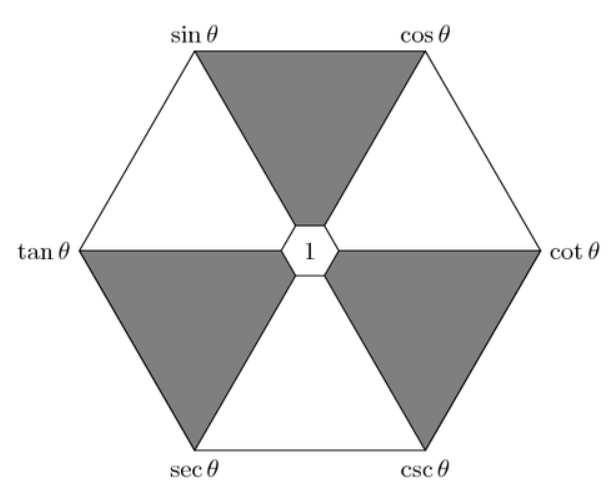
\includegraphics[width=0.5\linewidth]{Images/trighex.png}
    \caption{Trigonometric Identities Hexagon}
    \label{fig:enter-label}
\end{figure}


   

The trigonometric identities hexagon is a visual tool that allows you to quickly identify the relationships between the six main trigonometric functions: \(\sin(\theta)\), \(\cos(\theta)\), \(\tan(\theta)\), \(\cot(\theta)\), \(\sec(\theta)\), and \(\csc(\theta)\). Here’s how you can use this hexagon:

\begin{itemize}
    \item \textbf{Reciprocal Identities:} The edges of the hexagon connect pairs of functions that are reciprocals of each other. For example, \(\sin(\theta)\) is connected to \(\csc(\theta)\) because \(\csc(\theta) = \frac{1}{\sin(\theta)}\). Similarly, \(\cos(\theta)\) is connected to \(\sec(\theta)\), and \(\tan(\theta)\) is connected to \(\cot(\theta)\).
    
    \item \textbf{Quotient Identities:} The diagonals of the hexagon represent the quotient identities. For instance, the diagonal connecting \(\sin(\theta)\) and \(\cos(\theta)\) corresponds to the identity \(\tan(\theta) = \frac{\sin(\theta)}{\cos(\theta)}\). Similarly, the diagonal between \(\tan(\theta)\) and \(\sec(\theta)\) reflects the identity \(\tan(\theta) = \frac{\sin(\theta)}{\cos(\theta)}\) when combined with the reciprocal identity \(\sec(\theta) = \frac{1}{\cos(\theta)}\).
    
    \item \textbf{Pythagorean Identities:} The hexagon also encodes the Pythagorean identities, which can be derived by combining the relationships around the hexagon. For example, starting from the identity \(\sin^2(\theta) + \cos^2(\theta) = 1\), you can use the quotient identity \(\tan(\theta) = \frac{\sin(\theta)}{\cos(\theta)}\) to derive \(1 + \tan^2(\theta) = \sec^2(\theta)\). A similar process can be applied using \(\cot(\theta)\) and \(\csc(\theta)\) to derive the identity \(1 + \cot^2(\theta) = \csc^2(\theta)\).
\end{itemize}

By using the hexagon, you can easily recall or derive fundamental trigonometric identities without having to memorize each one individually. The geometric layout of the hexagon reveals the inherent symmetries and relationships between the functions, making it a valuable tool for both learning and applying trigonometry.


\section{Integration}
Below is the table of commonly seen integration.

\begin{table}[h]
\centering
\caption{Comprehensive Integration Table}
\begin{tabular}{ll ll}
\toprule
\text{Function } \(f(x)\) & \(\int f(x)\,dx\) & \text{Function } \(f(x)\) & \(\int f(x)\,dx\) \\
\midrule
\(x^n \ (n \neq -1)\) & \(\frac{x^{n+1}}{n+1} + C\) & \(\frac{1}{1+x^2}\) & \(\arctan x + C\) \\
\(\frac{1}{x}\) & \(\ln|x| + C\) & \(\frac{1}{\sqrt{1-x^2}}\) & \(\arcsin x + C\) \\
\(e^x\) & \(e^x + C\) & \(\frac{1}{\sqrt{x^2+a^2}}\) & \(\ln\left(x + \sqrt{x^2+a^2}\right) + C\) \\
\(a^x\) & \(\frac{a^x}{\ln a} + C\) & \(\frac{1}{\sqrt{x^2-a^2}}\) & \(\ln\left|x + \sqrt{x^2-a^2}\right| + C\) \\
\(\ln x\) & \(x\ln x - x + C\) & \(\frac{1}{a^2-x^2}\) & \(\frac{1}{2a}\ln\left|\frac{a+x}{a-x}\right| + C\) \\
\(\sin x\) & \(-\cos x + C\) & \(\arcsin x\) & \(x\arcsin x + \sqrt{1-x^2} + C\) \\
\(\cos x\) & \(\sin x + C\) & \(\arccos x\) & \(x\arccos x - \sqrt{1-x^2} + C\) \\
\(\tan x\) & \(-\ln|\cos x| + C\) & \(\arctan x\) & \(x\arctan x - \frac{1}{2}\ln(1+x^2) + C\) \\
\(\cot x\) & \(\ln|\sin x| + C\) & \(\text{arccot } x\) & \(x\text{ arccot} x + \frac{1}{2}\ln(1+x^2) + C\) \\
\(\sec x\) & \(\ln|\sec x + \tan x| + C\) & \(\text{arcsec } x\) & \(x\text{ arcsec} x - \ln|x + \sqrt{x^2-1}| + C\) \\
\(\csc x\) & \(-\ln|\csc x + \cot x| + C\) & \(\text{arccsc } x\) & \(x\text{ arccsc} x + \ln|x + \sqrt{x^2-1}| + C\) \\
\(\sec^2 x\) & \(\tan x + C\) & \(\sinh x\) & \(\cosh x + C\) \\
\(\csc^2 x\) & \(-\cot x + C\) & \(\cosh x\) & \(\sinh x + C\) \\
\(\sec x \tan x\) & \(\sec x + C\) & \(\tanh x\) & \(\ln(\cosh x) + C\) \\
\(\csc x \cot x\) & \(-\csc x + C\) & \(\coth x\) & \(\ln|\sinh x| + C\) \\
\bottomrule
\end{tabular}
\end{table}



\subsection{Integration Techniques}

\subsubsection{Integration by Parts}

\begin{definition}
Integration by parts is a technique based on the product rule of differentiation. It is useful when integrating the product of two functions.


$$
\int u \frac{dv}{dx} dx = uv - \int v \frac{du}{dx} dx
$$
Or alternatively:

$$\int u d v=u v-\int v d u$$

\end{definition}

\begin{theorem}[Proof of Integration by Parts]
Let $u = u(x)$ and $v = v(x)$. By the product rule:

$$
\frac{d}{dx}(uv) = u\frac{dv}{dx} + v\frac{du}{dx}
$$

Integrating both sides:

$$
\int \frac{d}{dx}(uv) dx = \int u\frac{dv}{dx} dx + \int v\frac{du}{dx} dx
$$

The left side simplifies to $uv$, and rearranging gives us the integration by parts formula.
\end{theorem}

\begin{exercise}
Evaluate the integral: $\int x^2 e^x \, dx$.

\end{exercise}
\begin{solution}
To solve this integral, we will use integration by parts twice. Let
\[
u = x^2 \quad \text{and} \quad dv = e^x \, dx
\]
then \( du = 2x \, dx \) and \( v = e^x \).

Applying integration by parts:
\[
\int x^2 e^x \, dx = x^2 e^x - \int 2x e^x \, dx
\]

Now, we need to evaluate \( \int 2x e^x \, dx \) using integration by parts again. Let
\[
u = 2x \quad \text{and} \quad dv = e^x \, dx
\]
then \( du = 2 \, dx \) and \( v = e^x \).

Thus,
\[
\int 2x e^x \, dx = 2x e^x - \int 2 e^x \, dx = 2x e^x - 2 e^x
\]

Substitute back:
\[
\int x^2 e^x \, dx = x^2 e^x - (2x e^x - 2 e^x)
\]
\[
= x^2 e^x - 2x e^x + 2 e^x
\]

So the final answer is:
\[
\int x^2 e^x \, dx = e^x (x^2 - 2x + 2) + C
\]
\end{solution}

\begin{exercise}
Evaluate the integral: $\int e^x \cos(x) \, dx$.
\end{exercise}
\begin{solution}
To solve this integral, we will use integration by parts twice and then solve for the integral. Let
\[
u = \cos(x) \quad \text{and} \quad dv = e^x \, dx
\]
then \( du = -\sin(x) \, dx \) and \( v = e^x \).

Applying integration by parts:
\[
\int e^x \cos(x) \, dx = e^x \cos(x) - \int e^x (-\sin(x)) \, dx
\]
\[
= e^x \cos(x) + \int e^x \sin(x) \, dx
\]

Now, we need to evaluate \( \int e^x \sin(x) \, dx \) using integration by parts again. Let
\[
u = \sin(x) \quad \text{and} \quad dv = e^x \, dx
\]
then \( du = \cos(x) \, dx \) and \( v = e^x \).

Thus,
\[
\int e^x \sin(x) \, dx = e^x \sin(x) - \int e^x \cos(x) \, dx
\]

Substituting back into the original equation:
\[
\int e^x \cos(x) \, dx = e^x \cos(x) + (e^x \sin(x) - \int e^x \cos(x) \, dx)
\]
\[
= e^x \cos(x) + e^x \sin(x) - \int e^x \cos(x) \, dx
\]

Now we have:
\[
\int e^x \cos(x) \, dx = e^x (\cos(x) + \sin(x)) - \int e^x \cos(x) \, dx
\]

Add \( \int e^x \cos(x) \, dx \) to both sides:
\[
2 \int e^x \cos(x) \, dx = e^x (\cos(x) + \sin(x))
\]

Divide by 2:
\[
\int e^x \cos(x) \, dx = \frac{e^x (\cos(x) + \sin(x))}{2} + C
\]
\end{solution}


\subsubsection{Integration by Substitution}

\begin{definition}
Integration by substitution is based on the chain rule of differentiation.

Formula:
If $u = g(x)$, then:

$$
\int f(g(x))g'(x)dx = \int f(u)du
$$
\end{definition}

\begin{theorem}[Proof of Integration by Substitution]
Let $F$ be an antiderivative of $f$. Then:

$$
\frac{d}{dx}[F(g(x))] = F'(g(x))g'(x) = f(g(x))g'(x)
$$

Integrating both sides:

$$
\int \frac{d}{dx}[F(g(x))] dx = \int f(g(x))g'(x)dx
$$

The left side simplifies to $F(g(x))$, which is equivalent to $\int f(u)du$ when we substitute $u = g(x)$.
\end{theorem}


\subsubsection{Trigonometric and Hyperbolic Function Substitution}

\begin{definition}
Trigonometric and hyperbolic function substitutions are specific techniques used for integrals involving expressions such as $\sqrt{a^2 - x^2}$, $\sqrt{a^2 + x^2}$, or $\sqrt{x^2 - a^2}$. These substitutions simplify the integral by transforming it into a form that is often easier to evaluate, depending on key identities associated with trigonometric or hyperbolic functions.

\begin{itemize}
    \item For $\sqrt{a^2 - x^2}$:
    \begin{itemize}
        \item Use $x = a\sin\theta$, where $\theta$ is a trigonometric angle. This substitution relies on the Pythagorean identity $\sin^2\theta + \cos^2\theta = 1$.
        \item Alternatively, use $x = a\tanh u$, where $u$ is a hyperbolic angle. This substitution depends on the hyperbolic identity $\cosh^2 u - \sinh^2 u = 1$.
    \end{itemize}
    
    \item For $\sqrt{a^2 + x^2}$:
    \begin{itemize}
        \item Use $x = a\tan\theta$, where $\theta$ is a trigonometric angle. This substitution is based on the identity $1 + \tan^2\theta = \sec^2\theta$.
        \item Alternatively, use $x = a\sinh u$, where $u$ is a hyperbolic angle. This substitution relies on the identity $\cosh^2 u - \sinh^2 u = 1$, specifically using the rearrangement $\cosh^2 u = 1 + \sinh^2 u$.
    \end{itemize}
    
    \item For $\sqrt{x^2 - a^2}$:
    \begin{itemize}
        \item Use $x = a\sec\theta$, where $\theta$ is a trigonometric angle. This substitution depends on the identity $\sec^2\theta - \tan^2\theta = 1$.
        \item Alternatively, use $x = a\cosh u$, where $u$ is a hyperbolic angle. This substitution is grounded in the identity $\cosh^2 u - \sinh^2 u = 1$.
    \end{itemize}
\end{itemize}
\end{definition}


\begin{example}[Substitution for $\sqrt{a^2 - x^2}$]
Using trigonometric substitution, let $x = a\sin\theta$. Then $dx = a\cos\theta \, d\theta$ and $\sqrt{a^2 - x^2} = a\cos\theta$.


Substituting $x = a\sin\theta$ into $\sqrt{a^2 - x^2}$:

$$
\sqrt{a^2 - (a\sin\theta)^2} = \sqrt{a^2(1 - \sin^2\theta)} = a\sqrt{\cos^2\theta} = a\cos\theta
$$

Alternatively, using hyperbolic substitution, let $x = a\tanh u$. Then $dx = a\text{sech}^2 u \, du$ and $\sqrt{a^2 - x^2} = \frac{a}{\cosh u}$.


Substituting $x = a\tanh u$ into $\sqrt{a^2 - x^2}$:

$$
\sqrt{a^2 - (a\tanh u)^2} = \sqrt{a^2\left(1 - \tanh^2 u\right)} = a\sqrt{\text{sech}^2 u} = \frac{a}{\cosh u}
$$
\end{example}

\begin{example}[Substitution for $\sqrt{a^2 + x^2}$]
Using trigonometric substitution, let $x = a\tan\theta$. Then $dx = a\sec^2\theta \, d\theta$ and $\sqrt{a^2 + x^2} = a\sec\theta$.

Proof:
Substituting $x = a\tan\theta$ into $\sqrt{a^2 + x^2}$:

$$
\sqrt{a^2 + (a\tan\theta)^2} = \sqrt{a^2(1 + \tan^2\theta)} = a\sqrt{\sec^2\theta} = a\sec\theta
$$

Alternatively, using hyperbolic substitution, let $x = a\sinh u$. Then $dx = a\cosh u \, du$ and $\sqrt{a^2 + x^2} = a\cosh u$.

Proof:
Substituting $x = a\sinh u$ into $\sqrt{a^2 + x^2}$:

$$
\sqrt{(a\sinh u)^2 + a^2} = \sqrt{a^2\sinh^2 u + a^2} = a\sqrt{\sinh^2 u + 1} = a\cosh u
$$
\end{example}

\begin{example}[Substitution for $\sqrt{x^2 - a^2}$]
Using trigonometric substitution, let $x = a\sec\theta$. Then $dx = a\sec\theta\tan\theta \, d\theta$ and $\sqrt{x^2 - a^2} = a\tan\theta$.

Proof:
Substituting $x = a\sec\theta$ into $\sqrt{x^2 - a^2}$:

$$
\sqrt{(a\sec\theta)^2 - a^2} = \sqrt{a^2\sec^2\theta - a^2} = a\sqrt{\sec^2\theta - 1} = a\tan\theta
$$

Alternatively, using hyperbolic substitution, let $x = a\cosh u$. Then $dx = a\sinh u \, du$ and $\sqrt{x^2 - a^2} = a\sinh u$.

Proof:
Substituting $x = a\cosh u$ into $\sqrt{x^2 - a^2}$:

$$
\sqrt{(a\cosh u)^2 - a^2} = \sqrt{a^2\cosh^2 u - a^2} = a\sqrt{\cosh^2 u - 1} = a\sinh u
$$
\end{example}

\subsubsection{Important Hyperbolic Function Identities}
Here are some important properties of hyperbolic functions. Most of them are quite similar, or even identical to trigonometric functions, however, do note that there are a lot of nuances.
\begin{table}[h]
\centering
\begin{tabular}{@{}ll@{}}
\toprule
Identity & Formula \\
\midrule
Pythagorean & $\cosh^2 x - \sinh^2 x = 1$ \\
 & $\tanh^2 x + \text{sech}^2 x = 1$ \\
 & $\coth^2 x - \text{csch}^2 x = 1$ \\
\midrule
Reciprocal & $\text{sech} \, x = \frac{1}{\cosh x}$, $\text{csch} \, x = \frac{1}{\sinh x}$ \\
 & $\coth x = \frac{1}{\tanh x}$ \\
\midrule
Quotient & $\tanh x = \frac{\sinh x}{\cosh x}$, $\coth x = \frac{\cosh x}{\sinh x}$ \\
\midrule
Even-Odd & $\sinh(-x) = -\sinh x$, $\cosh(-x) = \cosh x$ \\
 & $\tanh(-x) = -\tanh x$, $\coth(-x) = -\coth x$ \\
\midrule
Periodicity & $\sinh(x + 2\pi i) = \sinh x$, $\cosh(x + 2\pi i) = \cosh x$ \\
 & $\tanh(x + \pi i) = \tanh x$ \\
\bottomrule
\end{tabular}
\caption{Basic Hyperbolic Function Identities}
\label{tab:basic_hyperbolic_identities}
\end{table}

\begin{table}[h]
\centering
\begin{tabular}{@{}ll@{}}
\toprule
Identity & Formula \\
\midrule
Sum & $\sinh(A + B) = \sinh A \cosh B + \cosh A \sinh B$ \\
 & $\cosh(A + B) = \cosh A \cosh B + \sinh A \sinh B$ \\
 & $\tanh(A + B) = \frac{\tanh A + \tanh B}{1 + \tanh A \tanh B}$ \\
\midrule
Difference & $\sinh(A - B) = \sinh A \cosh B - \cosh A \sinh B$ \\
 & $\cosh(A - B) = \cosh A \cosh B - \sinh A \sinh B$ \\
 & $\tanh(A - B) = \frac{\tanh A - \tanh B}{1 - \tanh A \tanh B}$ \\
\midrule
Double Angle & $\sinh 2x = 2\sinh x \cosh x$ \\
 & $\cosh 2x = \cosh^2 x + \sinh^2 x = 2\cosh^2 x - 1 = 1 + 2\sinh^2 x$ \\
 & $\tanh 2x = \frac{2\tanh x}{1 + \tanh^2 x}$ \\
\midrule
Half Angle & $\sinh^2 \frac{x}{2} = \frac{\cosh x - 1}{2}$ \\
 & $\cosh^2 \frac{x}{2} = \frac{\cosh x + 1}{2}$ \\
 & $\tanh^2 \frac{x}{2} = \frac{\cosh x - 1}{\cosh x + 1}$ \\
\bottomrule
\end{tabular}
\caption{Advanced Hyperbolic Function Identities}
\label{tab:advanced_hyperbolic_identities}
\end{table}

\begin{table}[h]
\centering
\begin{tabular}{@{}ll@{}}
\toprule
Identity & Formula \\
\midrule
Product-to-Sum & $\sinh A \cosh B = \frac{1}{2}[\sinh(A + B) + \sinh(A - B)]$ \\
 & $\cosh A \cosh B = \frac{1}{2}[\cosh(A + B) + \cosh(A - B)]$ \\
 & $\sinh A \sinh B = \frac{1}{2}[\cosh(A + B) - \cosh(A - B)]$ \\
\midrule
Sum-to-Product & $\sinh A + \sinh B = 2 \sinh(\frac{A + B}{2}) \cosh(\frac{A - B}{2})$ \\
 & $\cosh A + \cosh B = 2 \cosh(\frac{A + B}{2}) \cosh(\frac{A - B}{2})$ \\
 & $\sinh A - \sinh B = 2 \cosh(\frac{A + B}{2}) \sinh(\frac{A - B}{2})$ \\
\bottomrule
\end{tabular}
\caption{Product-to-Sum and Sum-to-Product Hyperbolic Identities}
\label{tab:product_sum_hyperbolic_identities}
\end{table}